% Options for packages loaded elsewhere
\PassOptionsToPackage{unicode}{hyperref}
\PassOptionsToPackage{hyphens}{url}
%
\documentclass[
]{book}
\usepackage{amsmath,amssymb}
\usepackage{lmodern}
\usepackage{iftex}
\ifPDFTeX
  \usepackage[T1]{fontenc}
  \usepackage[utf8]{inputenc}
  \usepackage{textcomp} % provide euro and other symbols
\else % if luatex or xetex
  \usepackage{unicode-math}
  \defaultfontfeatures{Scale=MatchLowercase}
  \defaultfontfeatures[\rmfamily]{Ligatures=TeX,Scale=1}
\fi
% Use upquote if available, for straight quotes in verbatim environments
\IfFileExists{upquote.sty}{\usepackage{upquote}}{}
\IfFileExists{microtype.sty}{% use microtype if available
  \usepackage[]{microtype}
  \UseMicrotypeSet[protrusion]{basicmath} % disable protrusion for tt fonts
}{}
\makeatletter
\@ifundefined{KOMAClassName}{% if non-KOMA class
  \IfFileExists{parskip.sty}{%
    \usepackage{parskip}
  }{% else
    \setlength{\parindent}{0pt}
    \setlength{\parskip}{6pt plus 2pt minus 1pt}}
}{% if KOMA class
  \KOMAoptions{parskip=half}}
\makeatother
\usepackage{xcolor}
\usepackage{color}
\usepackage{fancyvrb}
\newcommand{\VerbBar}{|}
\newcommand{\VERB}{\Verb[commandchars=\\\{\}]}
\DefineVerbatimEnvironment{Highlighting}{Verbatim}{commandchars=\\\{\}}
% Add ',fontsize=\small' for more characters per line
\usepackage{framed}
\definecolor{shadecolor}{RGB}{248,248,248}
\newenvironment{Shaded}{\begin{snugshade}}{\end{snugshade}}
\newcommand{\AlertTok}[1]{\textcolor[rgb]{0.94,0.16,0.16}{#1}}
\newcommand{\AnnotationTok}[1]{\textcolor[rgb]{0.56,0.35,0.01}{\textbf{\textit{#1}}}}
\newcommand{\AttributeTok}[1]{\textcolor[rgb]{0.77,0.63,0.00}{#1}}
\newcommand{\BaseNTok}[1]{\textcolor[rgb]{0.00,0.00,0.81}{#1}}
\newcommand{\BuiltInTok}[1]{#1}
\newcommand{\CharTok}[1]{\textcolor[rgb]{0.31,0.60,0.02}{#1}}
\newcommand{\CommentTok}[1]{\textcolor[rgb]{0.56,0.35,0.01}{\textit{#1}}}
\newcommand{\CommentVarTok}[1]{\textcolor[rgb]{0.56,0.35,0.01}{\textbf{\textit{#1}}}}
\newcommand{\ConstantTok}[1]{\textcolor[rgb]{0.00,0.00,0.00}{#1}}
\newcommand{\ControlFlowTok}[1]{\textcolor[rgb]{0.13,0.29,0.53}{\textbf{#1}}}
\newcommand{\DataTypeTok}[1]{\textcolor[rgb]{0.13,0.29,0.53}{#1}}
\newcommand{\DecValTok}[1]{\textcolor[rgb]{0.00,0.00,0.81}{#1}}
\newcommand{\DocumentationTok}[1]{\textcolor[rgb]{0.56,0.35,0.01}{\textbf{\textit{#1}}}}
\newcommand{\ErrorTok}[1]{\textcolor[rgb]{0.64,0.00,0.00}{\textbf{#1}}}
\newcommand{\ExtensionTok}[1]{#1}
\newcommand{\FloatTok}[1]{\textcolor[rgb]{0.00,0.00,0.81}{#1}}
\newcommand{\FunctionTok}[1]{\textcolor[rgb]{0.00,0.00,0.00}{#1}}
\newcommand{\ImportTok}[1]{#1}
\newcommand{\InformationTok}[1]{\textcolor[rgb]{0.56,0.35,0.01}{\textbf{\textit{#1}}}}
\newcommand{\KeywordTok}[1]{\textcolor[rgb]{0.13,0.29,0.53}{\textbf{#1}}}
\newcommand{\NormalTok}[1]{#1}
\newcommand{\OperatorTok}[1]{\textcolor[rgb]{0.81,0.36,0.00}{\textbf{#1}}}
\newcommand{\OtherTok}[1]{\textcolor[rgb]{0.56,0.35,0.01}{#1}}
\newcommand{\PreprocessorTok}[1]{\textcolor[rgb]{0.56,0.35,0.01}{\textit{#1}}}
\newcommand{\RegionMarkerTok}[1]{#1}
\newcommand{\SpecialCharTok}[1]{\textcolor[rgb]{0.00,0.00,0.00}{#1}}
\newcommand{\SpecialStringTok}[1]{\textcolor[rgb]{0.31,0.60,0.02}{#1}}
\newcommand{\StringTok}[1]{\textcolor[rgb]{0.31,0.60,0.02}{#1}}
\newcommand{\VariableTok}[1]{\textcolor[rgb]{0.00,0.00,0.00}{#1}}
\newcommand{\VerbatimStringTok}[1]{\textcolor[rgb]{0.31,0.60,0.02}{#1}}
\newcommand{\WarningTok}[1]{\textcolor[rgb]{0.56,0.35,0.01}{\textbf{\textit{#1}}}}
\usepackage{longtable,booktabs,array}
\usepackage{calc} % for calculating minipage widths
% Correct order of tables after \paragraph or \subparagraph
\usepackage{etoolbox}
\makeatletter
\patchcmd\longtable{\par}{\if@noskipsec\mbox{}\fi\par}{}{}
\makeatother
% Allow footnotes in longtable head/foot
\IfFileExists{footnotehyper.sty}{\usepackage{footnotehyper}}{\usepackage{footnote}}
\makesavenoteenv{longtable}
\usepackage{graphicx}
\makeatletter
\def\maxwidth{\ifdim\Gin@nat@width>\linewidth\linewidth\else\Gin@nat@width\fi}
\def\maxheight{\ifdim\Gin@nat@height>\textheight\textheight\else\Gin@nat@height\fi}
\makeatother
% Scale images if necessary, so that they will not overflow the page
% margins by default, and it is still possible to overwrite the defaults
% using explicit options in \includegraphics[width, height, ...]{}
\setkeys{Gin}{width=\maxwidth,height=\maxheight,keepaspectratio}
% Set default figure placement to htbp
\makeatletter
\def\fps@figure{htbp}
\makeatother
\setlength{\emergencystretch}{3em} % prevent overfull lines
\providecommand{\tightlist}{%
  \setlength{\itemsep}{0pt}\setlength{\parskip}{0pt}}
\setcounter{secnumdepth}{5}
\usepackage{booktabs}
\ifLuaTeX
  \usepackage{selnolig}  % disable illegal ligatures
\fi
\usepackage[]{natbib}
\bibliographystyle{plainnat}
\IfFileExists{bookmark.sty}{\usepackage{bookmark}}{\usepackage{hyperref}}
\IfFileExists{xurl.sty}{\usepackage{xurl}}{} % add URL line breaks if available
\urlstyle{same} % disable monospaced font for URLs
\hypersetup{
  pdftitle={Breaking the Ice with R and RStudio},
  pdfauthor={Gaston Sanchez},
  hidelinks,
  pdfcreator={LaTeX via pandoc}}

\title{Breaking the Ice with R and RStudio}
\author{Gaston Sanchez}
\date{}

\begin{document}
\maketitle

{
\setcounter{tocdepth}{1}
\tableofcontents
}
\hypertarget{about}{%
\chapter*{About}\label{about}}
\addcontentsline{toc}{chapter}{About}

\begin{center}
\includegraphics[width=0.5\linewidth]{images/R-ice-breaker-cover} \end{center}

This manuscript provides a brief tutorial for getting started with R and
RStudio.

\hypertarget{citation}{%
\subsubsection*{Citation}\label{citation}}
\addcontentsline{toc}{subsubsection}{Citation}

You can cite this work as:

Sanchez, G. (2022) Breaking the Ice with R and RStudio.
\url{https://www.gastonsanchez.com/R-ice-breaker}

\begin{center}\rule{0.5\linewidth}{0.5pt}\end{center}

\hypertarget{my-series-of-r-tutorials}{%
\subsection*{My Series of R Tutorials}\label{my-series-of-r-tutorials}}
\addcontentsline{toc}{subsection}{My Series of R Tutorials}

This document is part of series of texts that I've written about Programming
and Data Analysis in R:

\begin{itemize}
\tightlist
\item
  \textbf{Tidy Hurricanes: Analyzing Tropical Storms with Tidyverse Tools}
\end{itemize}

\url{https://www.gastonsanchez.com/R-tidy-hurricanes}

\begin{itemize}
\tightlist
\item
  \textbf{R Coding Basics: An Introduction to Practical Programming in R}
\end{itemize}

\url{https://www.gastonsanchez.com/R-coding-basics}

\begin{itemize}
\tightlist
\item
  \textbf{Rolling Dice: Exploring Simulations in Games of Chance with R}
\end{itemize}

\url{https://www.gastonsanchez.com/R-rolling-dice}

\begin{itemize}
\tightlist
\item
  \textbf{Web Technologies in R: A Short Introduction to Web Data Technologies in R}
\end{itemize}

\url{https://www.gastonsanchez.com/R-web-tech}

\begin{center}\rule{0.5\linewidth}{0.5pt}\end{center}

\hypertarget{donation}{%
\subsection*{Donation}\label{donation}}
\addcontentsline{toc}{subsection}{Donation}

As a Data Science and Statistics educator, I love to share the work I do. Each month I spend dozens of hours curating learning materials like this resource. If you find any value and usefulness in it, please consider making a one-time donation---via PayPal---in any amount (e.g.~the amount you would spend inviting me a cup of coffee or any other drink). Your support really matters.

\hypertarget{license}{%
\subsection*{License}\label{license}}
\addcontentsline{toc}{subsection}{License}

This work is licensed under a Creative Commons Attribution-NonCommercial-ShareAlike 4.0 International License.

\hypertarget{installing-r}{%
\chapter{Installing R}\label{installing-r}}

To learn how to use R, you obviously need to have access to it. This chapter,
and the next one, guide you through the installation process of R and RStudio
so that you can have both programs up and running in your computer.

If you already have R and RStudio installed in your machine, you can safely
go to chapter \protect\hyperlink{rintro}{First Contact with R}.

\hypertarget{interacting-with-r}{%
\section{Interacting with R}\label{interacting-with-r}}

Before I show you how to install R and the integrated development environment
RStudio, let me tell you first about the different ways in which users can
work with R.

Overall, you can work with R in two major ways:

\begin{enumerate}
\def\labelenumi{\arabic{enumi})}
\item
  Interactive Mode, and
\item
  Non-interactive Mode
\end{enumerate}

\textbf{Interactive Mode.} Most R users work with R in an interactive way, and this
is certainly the way I personally interact with R in my daily coding activities.
Interactive means that you launch R (i.e.~you open a session), having direct
access to its console. This is where you type in commands, and then R does its
magic reading the commands, parsing them, evaluating them,
and---typically---printing an output back into the console, waiting for you to
type in the next command(s).

\textbf{Non-interactive Mode.} In contrast to interactive mode, working with R in
non-interactive way involves writing all the commands in a text file (for
example in an \texttt{R} script file), and then asking your computer---via the
command line interface---to pass this file to R so that it runs the
commands without you launching R or having direct access to its console.

Think of interactive way as having a direct conversation with R, establishing
a dialogue in which you type in a command, R interprets it, gives you an
answer, and then you type more commands, continuing the dialogue. In contrast,
non-interactive is like writing a letter (or an email) to R. Here you don't
have that synchronous conversation, instead R will see the script file, try to
execute all the commands ``behind the scenes'', and it will disappear when it
finishes the computations. You may get some output back, but R is gone in the
sense that there is no open session waiting for you to execute the next
instructions.

Most of what I discuss in this book is applicable to writing code in R
regardless of how you decide to interact with R. However, to learn R and to
follow the examples of the book it is definitely much better to do it in an
interactive way using: a) R's built-in graphical user interface (R's GUI),
b) an integrated development environment (IDE) such as RStudio, or
c) R from a command line interface (CLI) commonly referred to as a \emph{terminal}.

\begin{figure}

{\centering 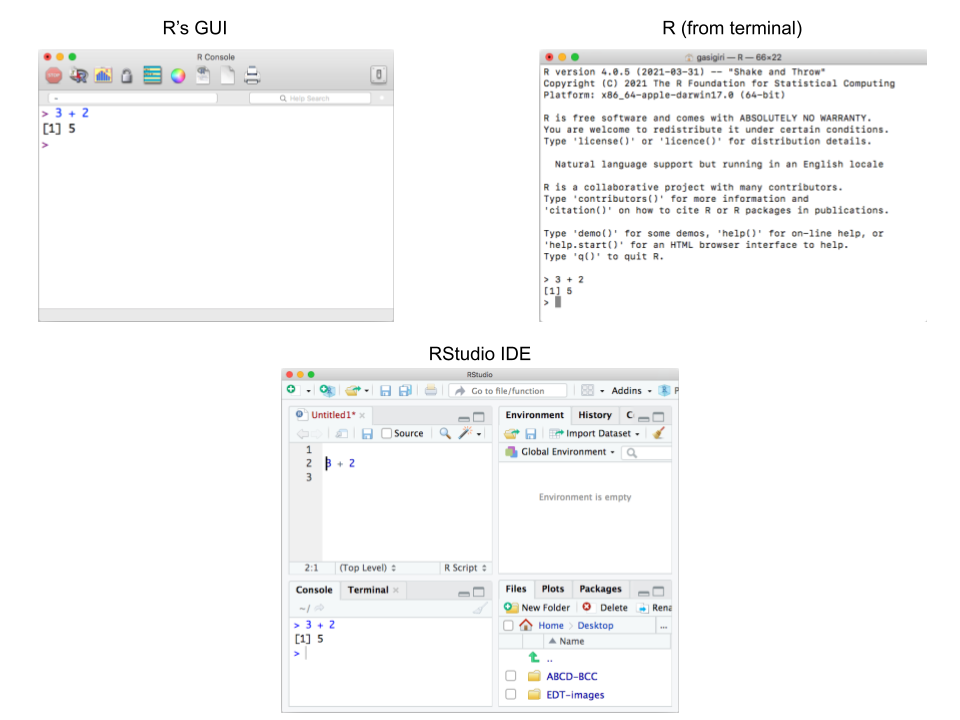
\includegraphics[width=0.9\linewidth]{images/install/r-interactive-ways} 

}

\caption{Interacting with R in various ways: R's GUI, RStudio, and R from a command-line terminal}\label{fig:unnamed-chunk-4}
\end{figure}

While you can interact with R using its built-in graphical user interface (GUI)
or launching R from the terminal (command line interface), nowadays I highly
recommend that you interact with it using an
\emph{Integrated Development Environment} (IDE) such as
\href{https://www.rstudio.com/}{\textbf{RStudio}}. Simply put,
programs like RStudio provide a nice working space that make your life easier
while writing code, creating all sorts of reports, documents, and slides,
running analysis, making graphs, generating outputs, creating web apps, etc.

\begin{figure}

{\centering 
\includegraphics[width=0.3\linewidth]{images/rstudio/r-rstudio-logos} 

}

\caption{Main computational tools: R and RStudio}\label{fig:unnamed-chunk-5}
\end{figure}

Keep in mind that R and RStudio are not the same thing. R is like the main\\
``engine'' or computational core. RStudio is just a convenient layer that
talks directly to R, and gives us a convenient working space to organize our
files, to type in code, to run commands, visualize plots, interact with our
filesystem, etc. Having said that, everything that happens in RStudio, can
be done in R alone. Yes, you may need to write more code and work in a more
rudimentary way, but nothing should stop your work in R if one day RStudio
disappears from the face of the earth.

By the way, both R and RStudio are free, and available for Mac (OS X), Windows,
and Linux (e.g.~Ubuntu, Fedora, Debian). More about this in the following
sections.

\hypertarget{installing-r-1}{%
\section{Installing R}\label{installing-r-1}}

To download and install R in your computer, follow the steps listed below.

\textbf{Step 1)} Go to the \textbf{R project} website: \url{https://r-project.org}

\begin{figure}

{\centering 
\includegraphics[width=0.7\linewidth]{images/install/r-project} 

}

\caption{R project's home webpage}\label{fig:unnamed-chunk-6}
\end{figure}

\textbf{Step 2)} Click on the CRAN link, located in the navigation bar (on the left
side). This will take you to the \emph{Comprehensive R Archive Network} page (see
screenshot below).

\begin{figure}

{\centering 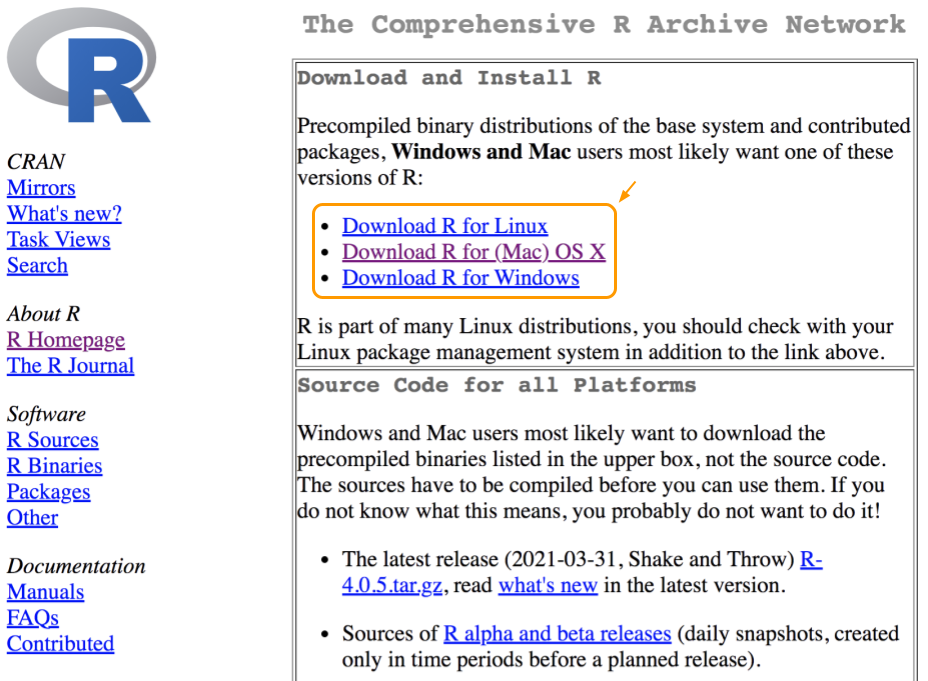
\includegraphics[width=0.7\linewidth]{images/install/cran-download} 

}

\caption{R is available for MacOS, Windows, and Linux}\label{fig:unnamed-chunk-7}
\end{figure}

\textbf{Step 3)} Click on the download option that corresponds to your operating
system (e.g.~Linux, Mac, or Windows). In my case, I have a Mac computer, which
explains why the Mac OS-X link is highlighted in the above screenshot.

\begin{figure}

{\centering 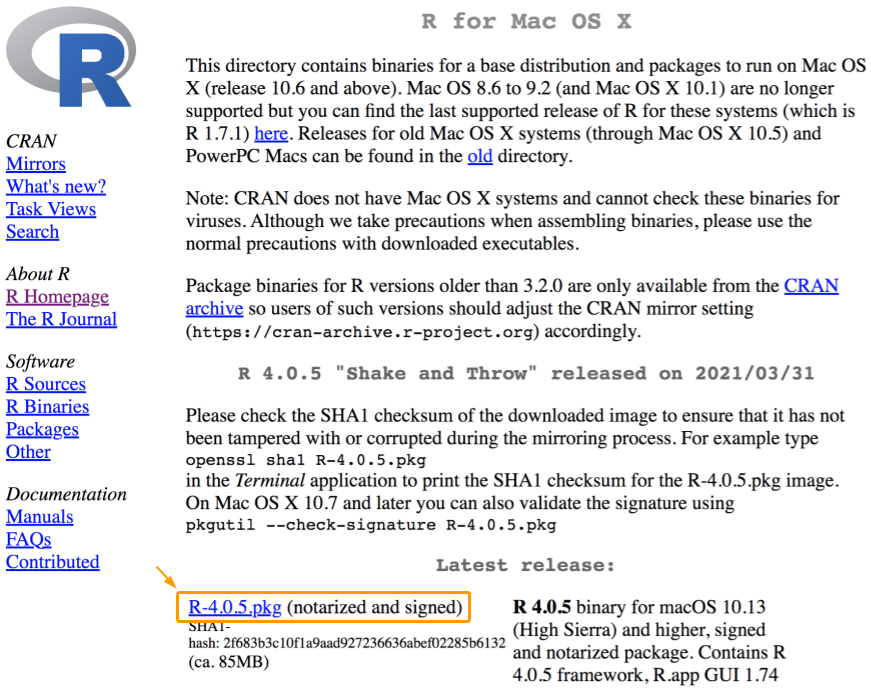
\includegraphics[width=0.7\linewidth]{images/install/cran-mac} 

}

\caption{CRAN download for Mac}\label{fig:unnamed-chunk-8}
\end{figure}

For most users, you will want to install the \textbf{Latest release}, which in the screenshot above happens to be \texttt{R\ 4.0.5\ "Shake\ and\ Throw"}. Keep in mind that
by the time you read this book, R will very likely have a more recent version.

\textbf{Step 4)} Click on the package link, which in the screenshot corresponds to
\texttt{R-4.0.5.pkg}. This is the link of a compressed file that contains the binary
code. Before installing a given version of R, read the
description of the release to make sure the operating system in your computer
is compatible with a specific version of R.

After clicking on the \texttt{R-4.0.5.pkg} link, the compressed file will be
downloaded to your computer.

\textbf{Step 5.} Click on the downloaded file. An installation wizard will open
automatically, ready to guide you through the installation process, step by
step (see image below).

\begin{figure}

{\centering 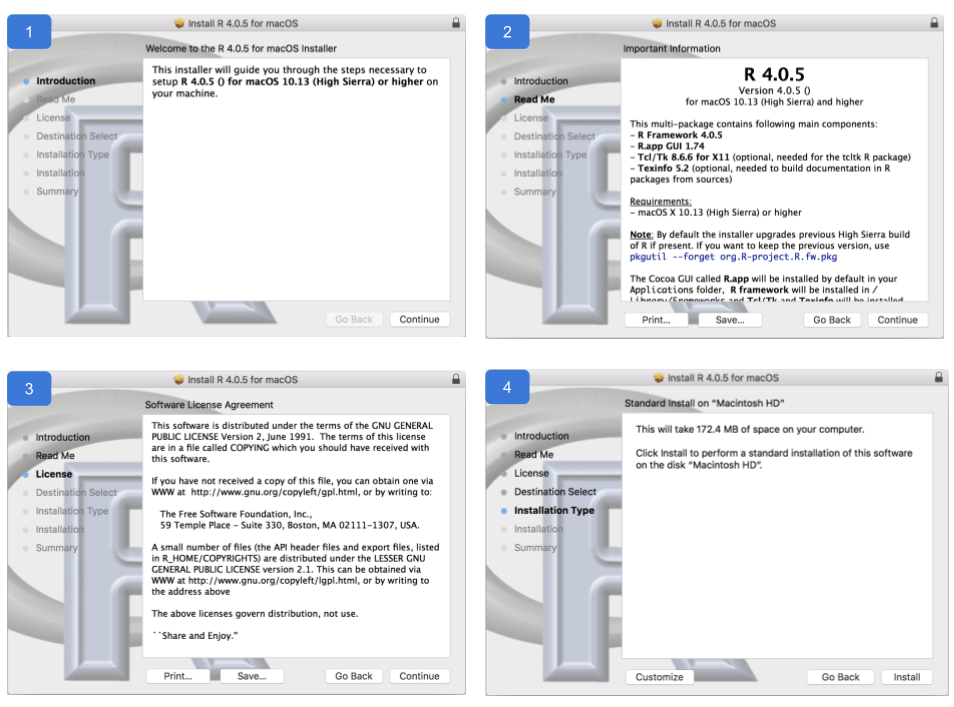
\includegraphics[width=0.9\linewidth]{images/install/R-install-steps} 

}

\caption{R Installation wizard for Mac}\label{fig:unnamed-chunk-9}
\end{figure}

In most cases, you will want to use the default settings. Personally, I've been
using the default settings for several years without having the need to
customize anything.

At the end of the installation, if everything went well, you should be able
to see a successful message (see figure below):

\begin{figure}

{\centering 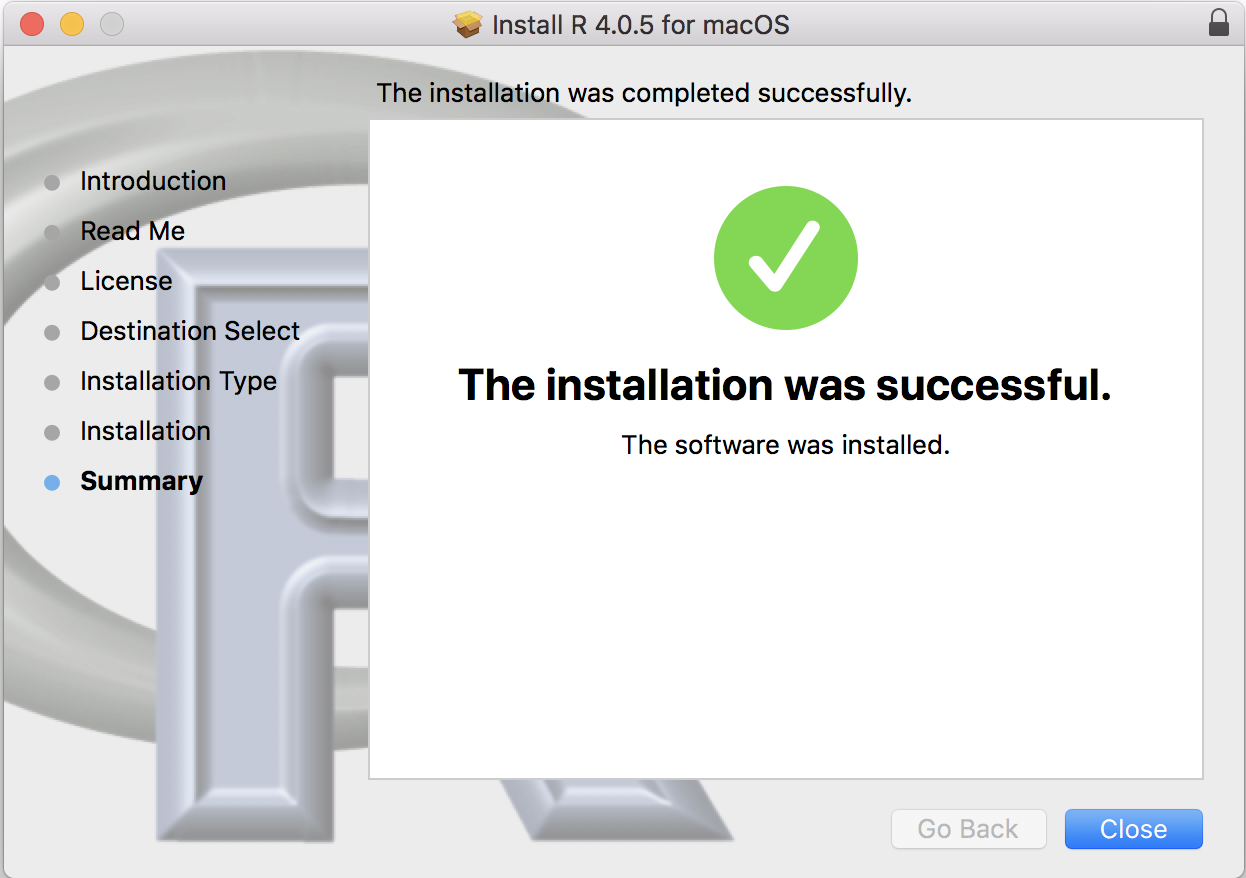
\includegraphics[width=0.5\linewidth]{images/install/install-5} 

}

\caption{R Installation wizard for Mac}\label{fig:unnamed-chunk-10}
\end{figure}

\hypertarget{installing-rstudio}{%
\chapter{Installing RStudio}\label{installing-rstudio}}

In addition to R, the other program you will need to have installed in your
machine is RStudio.

Technically speaking, RStudio is an \emph{Integrated Development Environment} (IDE)
developed by \href{https://posit.co}{Posit}. An IDE is just the fancy term that is
used for a program that provides a nice working space that make your life easier
while writing code, running analysis, and making graphs. In addition, you can
also use RStudio to create all sorts of reports, documents, slides, and web apps.

\hypertarget{download-rstudio}{%
\section{Download RStudio}\label{download-rstudio}}

To download the Desktop version of RStudio follow the steps listed below.

\textbf{Step 1)} Go to \textbf{Posit's} download webpage:

\url{https://posit.co/downloads/}

\begin{figure}

{\centering 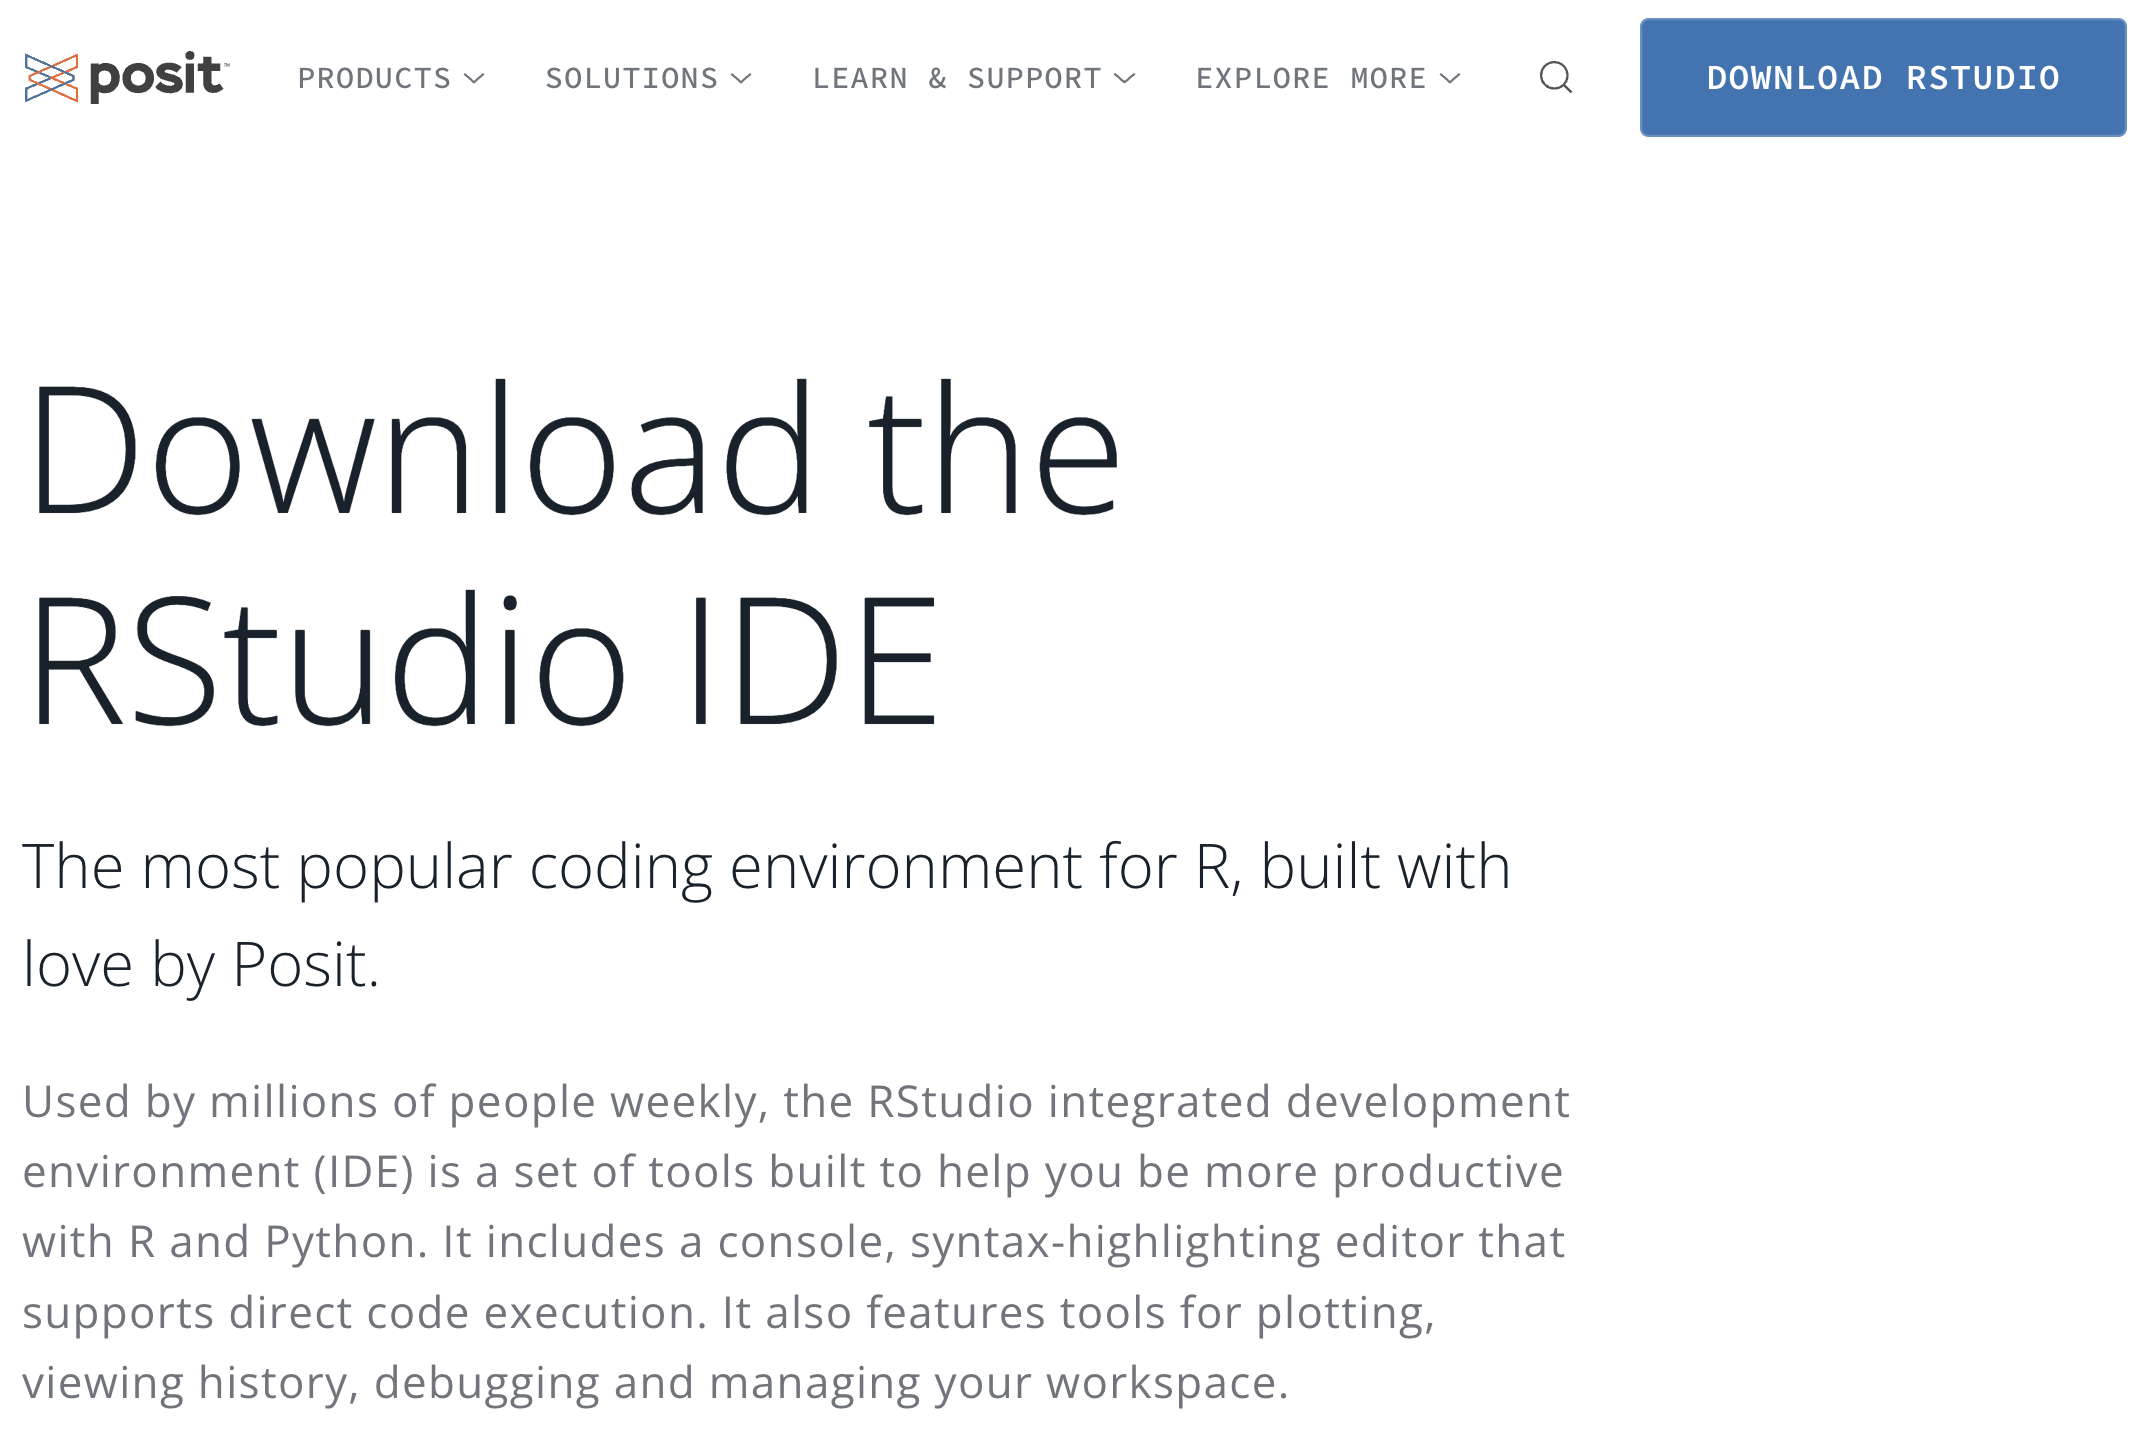
\includegraphics[width=0.7\linewidth]{images/install/posit-rstudio-download} 

}

\caption{RStudio download options}\label{fig:unnamed-chunk-12}
\end{figure}

At the time of this writing, there are two options of RStudio Desktop: 1) the
Free version, and 2) the Pro version.

\textbf{Step 2)} Choose the \textbf{Free} version of RStudio Desktop (see image below),
and click on the ``DOWNLOAD'' button.

\begin{figure}

{\centering 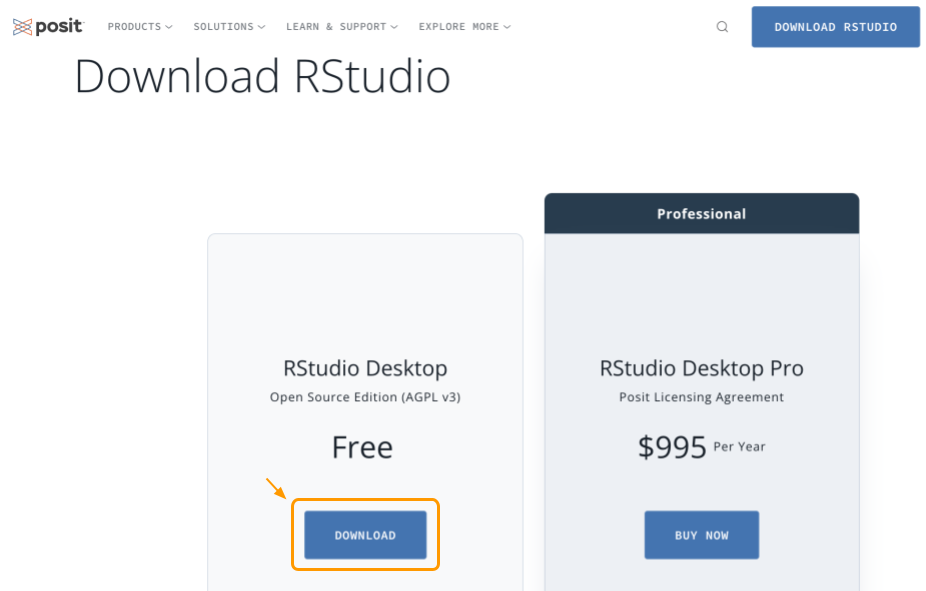
\includegraphics[width=0.7\linewidth]{images/install/posit-rstudio-free} 

}

\caption{Choose RStudio free desktop}\label{fig:unnamed-chunk-13}
\end{figure}

\textbf{Step 3)} Select the version that matches your operating system (e.g.~Windows,
macOS, linux). Double check that the operating system in your computer
is compatible with a specific version of RStudio.

\begin{figure}

{\centering 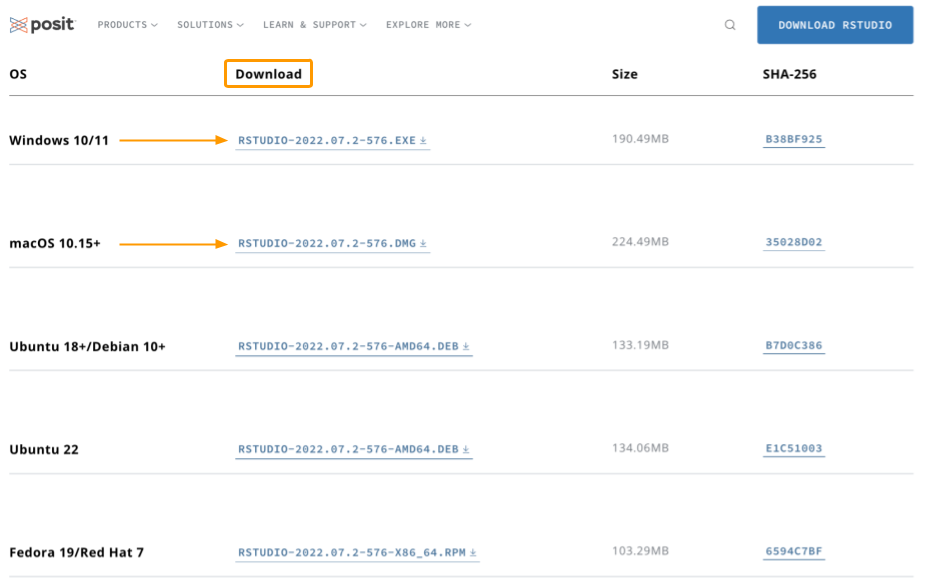
\includegraphics[width=0.7\linewidth]{images/install/posit-rstudio-versions} 

}

\caption{RStudio Desktop versions}\label{fig:unnamed-chunk-14}
\end{figure}

Once the installation of RStudio is completed, you should be able to open a new
session in RStudio, and start interacting with R.

\hypertarget{rintro}{%
\chapter{First Contact with R}\label{rintro}}

If you are new to R and don't have any programming experience, then you
should read this chapter in its entirety. If you already have some previous
experience working with R and/or have some programming background, then you may
want to skim over most of the introductory chapters of part I.

This chapter, and the rest of the book, assumes that you have installed both R
and RStudio in your computer. If this is not the case, then go to chapters
\protect\hyperlink{installing-r}{Installing R} and \protect\hyperlink{installing-rstudio}{Installing RStudio} to
follow the steps for downloading and installing these programs.

R comes with a simple built-in graphical user interface (GUI), and you can
certainly start working with it right out of the box. That is actually the way
I got my first contact with R back in 2001 during my senior year in college.
Nowadays, instead of using R's GUI, it is more convenient to interact with R
using a third party software such as RStudio.

I describe more introductory details about RStudio in the next chapter
\protect\hyperlink{rstudio}{A Quick Tour Around RStudio}. For now, go ahead and launch RStudio
in your computer.

\hypertarget{first-contact-with-r-via-rstudio}{%
\section{First Contact with R (via RStudio)}\label{first-contact-with-r-via-rstudio}}

When you open RStudio, you should be able to see its layout organized into
quadrants officially called \emph{panes}. The very first time you launch RStudio you
will only see three panes, like in the screenshot below.

\begin{figure}

{\centering 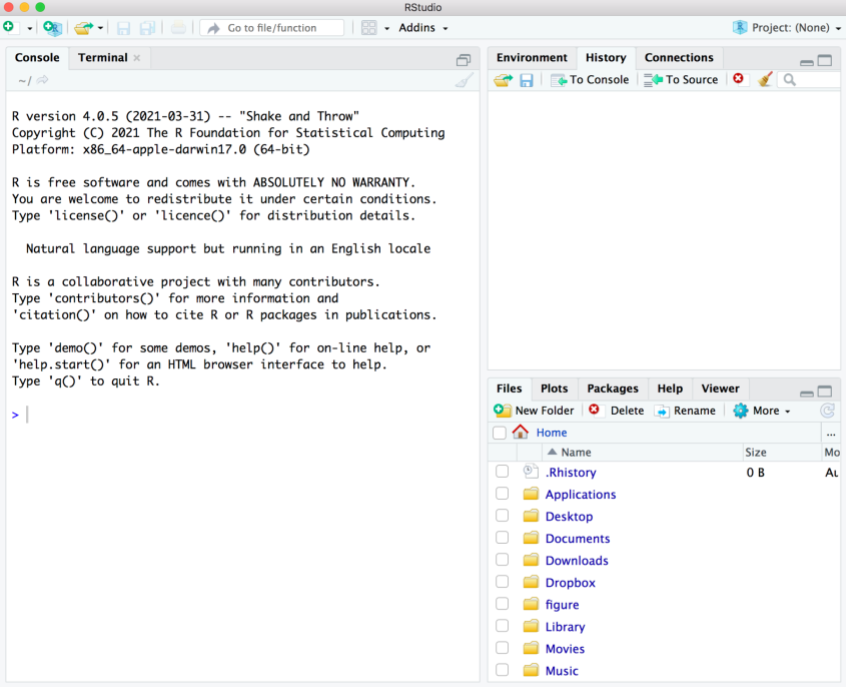
\includegraphics[width=0.7\linewidth]{images/rstudio/rstudio-launch-first-time} 

}

\caption{Screenshot of RStudio when launched for the first time.}\label{fig:unnamed-chunk-16}
\end{figure}

To help you break the ice with R, it's better if we start working directly
on the \textbf{Console}.

As you can tell from the following screenshot, the console is located in the
left-hand side quadrant of RStudio. Keep in mind that your RStudio's console
pane may be located in a different quadrant.

\begin{figure}

{\centering 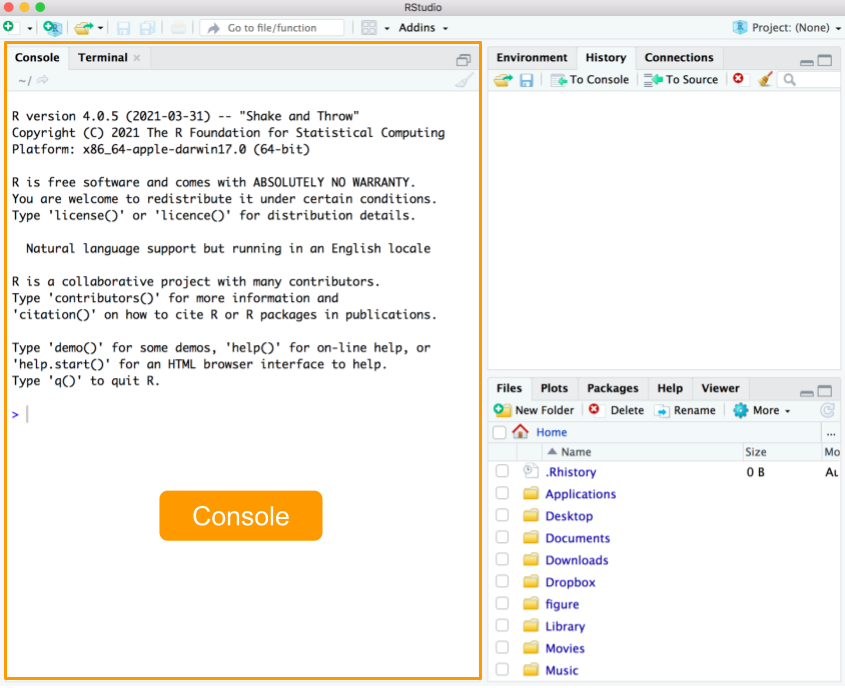
\includegraphics[width=0.7\linewidth]{images/rstudio/rstudio-console-first-time} 

}

\caption{Console quadrant in RStudio.}\label{fig:unnamed-chunk-17}
\end{figure}

Technically speaking, the console is a terminal where a user inputs commands and
views output. Simply put, this is where you can directly interact with R by
typing commands, and getting the output from the execution of the commands.

\hypertarget{r-as-a-scientific-calculator}{%
\subsection{R as a scientific calculator}\label{r-as-a-scientific-calculator}}

This first activity is dedicated for readers with little or no programming
experience, especially those of you who have never used software in which you
have to type commands. The idea is to start typing simple things in the
\textbf{console}, basically using R as a scientific calculator.

Here's a toy example. Consider the monthly bills of an undergraduate student:

\begin{itemize}
\tightlist
\item
  cell phone \$80
\item
  transportation \$20
\item
  groceries \$527
\item
  gym \$10
\item
  rent \$1500
\item
  other \$83
\end{itemize}

You can use R to find the student's total expenses by typing these commands in
the console:

\begin{Shaded}
\begin{Highlighting}[]
\DecValTok{80} \SpecialCharTok{+} \DecValTok{20} \SpecialCharTok{+} \DecValTok{527} \SpecialCharTok{+} \DecValTok{10} \SpecialCharTok{+} \DecValTok{1500} \SpecialCharTok{+} \DecValTok{83}
\end{Highlighting}
\end{Shaded}

There is nothing surprising or fancy about this piece of code. In fact, it has
all the numbers and all the \texttt{+} symbols that you would use if you had to obtain
the total expenses by using the calculator in your cellphone.

\hypertarget{assigning-values-to-objects}{%
\subsection{Assigning values to objects}\label{assigning-values-to-objects}}

Often, it will be more convenient to create \textbf{objects}, sometimes also called
\textbf{variables}, that store one or more values. To do this, type the name of the
object, followed by the assignment or ``arrow'' operator \texttt{\textless{}-}, followed by the
assigned value. By the way, the arrow operator consists of a left-angle bracket
\texttt{\textless{}} (or ``less than'' symbol) and a dash or hyphen symbol \texttt{-}.

For example, you can create an object \texttt{phone} to store the value of the monthly
cell phone bill, and then inspect the object by typing its name:

\begin{Shaded}
\begin{Highlighting}[]
\NormalTok{phone }\OtherTok{\textless{}{-}} \DecValTok{80}
\NormalTok{phone}
\SpecialCharTok{\textgreater{}}\NormalTok{ [}\DecValTok{1}\NormalTok{] }\DecValTok{80}
\end{Highlighting}
\end{Shaded}

All R statements where you create objects are known as \textbf{assignments}, and
they have this form:

\begin{Shaded}
\begin{Highlighting}[]
\NormalTok{object }\OtherTok{\textless{}{-}}\NormalTok{ value}
\end{Highlighting}
\end{Shaded}

this means you assign a \texttt{value} to a given \texttt{object}; one easy way to read the
previous assignment is ``phone gets 80''.

Alternatively, you can also use the equals sign \texttt{=} for assignments:

\begin{Shaded}
\begin{Highlighting}[]
\NormalTok{transportation }\OtherTok{=} \DecValTok{20}
\NormalTok{transportation}
\SpecialCharTok{\textgreater{}}\NormalTok{ [}\DecValTok{1}\NormalTok{] }\DecValTok{20}
\end{Highlighting}
\end{Shaded}

As you will see in the rest of the book, I've written most assignments with the
arrow operator \texttt{\textless{}-}. But you can perfectly replace them with the equals sign
\texttt{=}. The opposite is not necessarily true. There are some especial cases in
which an equals sign cannot be replaced with the arrow, but we'll talk about
this later.

\textbf{Pro tip.} RStudio has a keyboard shortcut for the arrow operator\texttt{\textless{}-}:

\begin{itemize}
\item
  Windows \& Linux users: \texttt{Alt} + \texttt{-}
\item
  Mac users: \texttt{Option} + \texttt{-}
\end{itemize}

In fact, there is a large set of keyboard shortcuts. In the menu bar, go to the
\emph{Help} tab, and then click on the option \emph{Keyboard Shorcuts Help} to find
information about all the available shortcuts.

\hypertarget{object-names}{%
\subsection{Object Names}\label{object-names}}

There are certain rules you have to follow when creating objects and variables.
Object names cannot start with a digit and cannot contain certain other characters
such as a comma or a space.

The following are invalid names (and invalid assignments)

\begin{Shaded}
\begin{Highlighting}[]
\CommentTok{\# cannot start with a number}
\NormalTok{5variable }\OtherTok{\textless{}{-}} \DecValTok{5}

\CommentTok{\# cannot start with an underscore}
\NormalTok{\_invalid }\OtherTok{\textless{}{-}} \DecValTok{10}

\CommentTok{\# cannot contain comma}
\NormalTok{my,variable }\OtherTok{\textless{}{-}} \DecValTok{3}

\CommentTok{\# cannot contain spaces}
\NormalTok{my variable }\OtherTok{\textless{}{-}} \DecValTok{1}
\end{Highlighting}
\end{Shaded}

People use different naming styles, and at some point you should also adopt a
convention for naming things. Some of the common styles are:

\begin{Shaded}
\begin{Highlighting}[]
\NormalTok{snake\_case}

\NormalTok{camelCase}

\NormalTok{period.case}
\end{Highlighting}
\end{Shaded}

Pretty much all the objects and variables that I create in this book follow the
``snake\_case'' style. It is certainly possible that you may end up working with
a team that has a style-guide with a specific naming convention. Feel free to try
various styles, and once you feel comfortable with one of them, then stick to it.

\hypertarget{case-sensitive}{%
\subsection{Case Sensitive}\label{case-sensitive}}

R is case sensitive. This means that \texttt{phone} is not the same as \texttt{Phone} or
\texttt{PHONE}

\begin{Shaded}
\begin{Highlighting}[]
\CommentTok{\# case sensitive}
\NormalTok{phone }\OtherTok{\textless{}{-}} \DecValTok{80}
\NormalTok{Phone }\OtherTok{\textless{}{-}} \SpecialCharTok{{-}}\DecValTok{80}
\NormalTok{PHONE }\OtherTok{\textless{}{-}} \DecValTok{8000}

\NormalTok{phone }\SpecialCharTok{+}\NormalTok{ Phone}
\SpecialCharTok{\textgreater{}}\NormalTok{ [}\DecValTok{1}\NormalTok{] }\DecValTok{0}

\NormalTok{PHONE }\SpecialCharTok{{-}}\NormalTok{ phone}
\SpecialCharTok{\textgreater{}}\NormalTok{ [}\DecValTok{1}\NormalTok{] }\DecValTok{7920}
\end{Highlighting}
\end{Shaded}

Again, this is one more reason why adopting a naming convention early on in
a data analysis or programming project is very important. Being consistent with
your notation may save you from some headaches down the road.

\hypertarget{calling-functions}{%
\subsection{Calling Functions}\label{calling-functions}}

Like any other programming language, R has many functions. To use a function
just type its name followed by parenthesis. Inside the parenthesis you
typically pass one or more inputs. Most functions will produce some type of
output:

\begin{Shaded}
\begin{Highlighting}[]
\CommentTok{\# absolute value}
\FunctionTok{abs}\NormalTok{(}\DecValTok{10}\NormalTok{)}
\FunctionTok{abs}\NormalTok{(}\SpecialCharTok{{-}}\DecValTok{4}\NormalTok{)}

\CommentTok{\# square root}
\FunctionTok{sqrt}\NormalTok{(}\DecValTok{9}\NormalTok{)}

\CommentTok{\# natural logarithm}
\FunctionTok{log}\NormalTok{(}\DecValTok{2}\NormalTok{)}
\end{Highlighting}
\end{Shaded}

In the above examples, the functions are taking a single input. But often you
will be working with functions that accept several inputs. The \texttt{log()} function
is one them. By default, \texttt{log()} computes the natural logarithm. But it also
has the \texttt{base} argument that allows you to specify the base of the logarithm,
say to \texttt{base\ =\ 10}

\begin{Shaded}
\begin{Highlighting}[]
\FunctionTok{log}\NormalTok{(}\DecValTok{10}\NormalTok{, }\AttributeTok{base =} \DecValTok{10}\NormalTok{)}
\SpecialCharTok{\textgreater{}}\NormalTok{ [}\DecValTok{1}\NormalTok{] }\DecValTok{1}
\end{Highlighting}
\end{Shaded}

\hypertarget{comments-in-r}{%
\subsection{Comments in R}\label{comments-in-r}}

All programming languages use a set of characters to indicate that a
specifc part or lines of code are \textbf{comments}, that is, things that are
not to be executed. R uses the hash or pound symbol \texttt{\#} to specify comments.
Any code to the right of \texttt{\#} will not be executed by R.

\begin{Shaded}
\begin{Highlighting}[]
\CommentTok{\# this is a comment}
\CommentTok{\# this is another comment}
\DecValTok{2} \SpecialCharTok{*} \DecValTok{9}

\DecValTok{4} \SpecialCharTok{+} \DecValTok{5}  \CommentTok{\# you can place comments like this}
\end{Highlighting}
\end{Shaded}

You will notice that I have included comments in almost all of the code
snippets shown in the book. To be honest, some examples may have too many
comments, but I've done that to be very explicit, and so that those of you
who lack coding experience understand what's going on. In real life, programmers
use comments, but not so much as I do in the book. The main purpose of
writing comments is to describe---conceptually---what is happening with certain
lines of code. Some would even argue that comments should only be used to
express not the what but the \textbf{why} a developer is doing something. In case
of doubt, especially if you don't have a lot of programming experience, I think
it's better to err on the side of caution by adding more comments than
including no comments whatsoever.

\hypertarget{help-documentation}{%
\section{Getting Help}\label{help-documentation}}

Because we work with functions all the time, it's important to know certain
details about how to use them, what input(s) is required, and what is the
returned output.

So how do you find all this information technically known as a function's
\textbf{documentation}? There are several ways to access this type of information.

If you know the name of a function you are interested in knowing more about,
you can use the function \texttt{help()} and pass it the name of the function you
are looking for:

\begin{Shaded}
\begin{Highlighting}[]
\CommentTok{\# documentation about the \textquotesingle{}abs\textquotesingle{} function}
\FunctionTok{help}\NormalTok{(abs)}

\CommentTok{\# documentation about the \textquotesingle{}mean\textquotesingle{} function}
\FunctionTok{help}\NormalTok{(mean)}
\end{Highlighting}
\end{Shaded}

Alternatively, you can use a shortcut using the question mark \texttt{?} followed
by the name of the function:

\begin{Shaded}
\begin{Highlighting}[]
\CommentTok{\# documentation about the \textquotesingle{}abs\textquotesingle{} function}
\NormalTok{?abs}

\CommentTok{\# documentation about the \textquotesingle{}mean\textquotesingle{} function}
\NormalTok{?mean}
\end{Highlighting}
\end{Shaded}

\texttt{help()} and \texttt{?} only work if you know the name of the function your are
looking for. Sometimes, however, you don't know the name of the function but
you may know some keyword(s). To look for related functions associated to a
keyword, use \texttt{help.search()} or simply type double question marks \texttt{??}

\begin{Shaded}
\begin{Highlighting}[]
\CommentTok{\# search for \textquotesingle{}absolute\textquotesingle{}}
\FunctionTok{help.search}\NormalTok{(}\StringTok{"absolute"}\NormalTok{)}

\CommentTok{\# alternatively you can also search like this:}
\NormalTok{??absolute}
\end{Highlighting}
\end{Shaded}

Notice the use of quotes surrounding the input name inside \texttt{help.search()}

Often overlooked by beginners but extremely helpful is to understand the
anatomy of the information displayed in the technical documentation. The
content is typically organized into seven sections listed below (although
sometimes there may be less or more sections)

\begin{itemize}
\tightlist
\item
  Title
\item
  Description
\item
  Usage of function
\item
  Arguments
\item
  Details
\item
  See Also
\item
  Examples
\end{itemize}

The three screenshots below show the ``Help'' or technical documentation of the
\texttt{log()} function. This information is in RStudio's \texttt{Help} tab, located in the
pane that contains other tabs such as \texttt{Files}, \texttt{Plots}, \texttt{Packages}.

\begin{figure}

{\centering 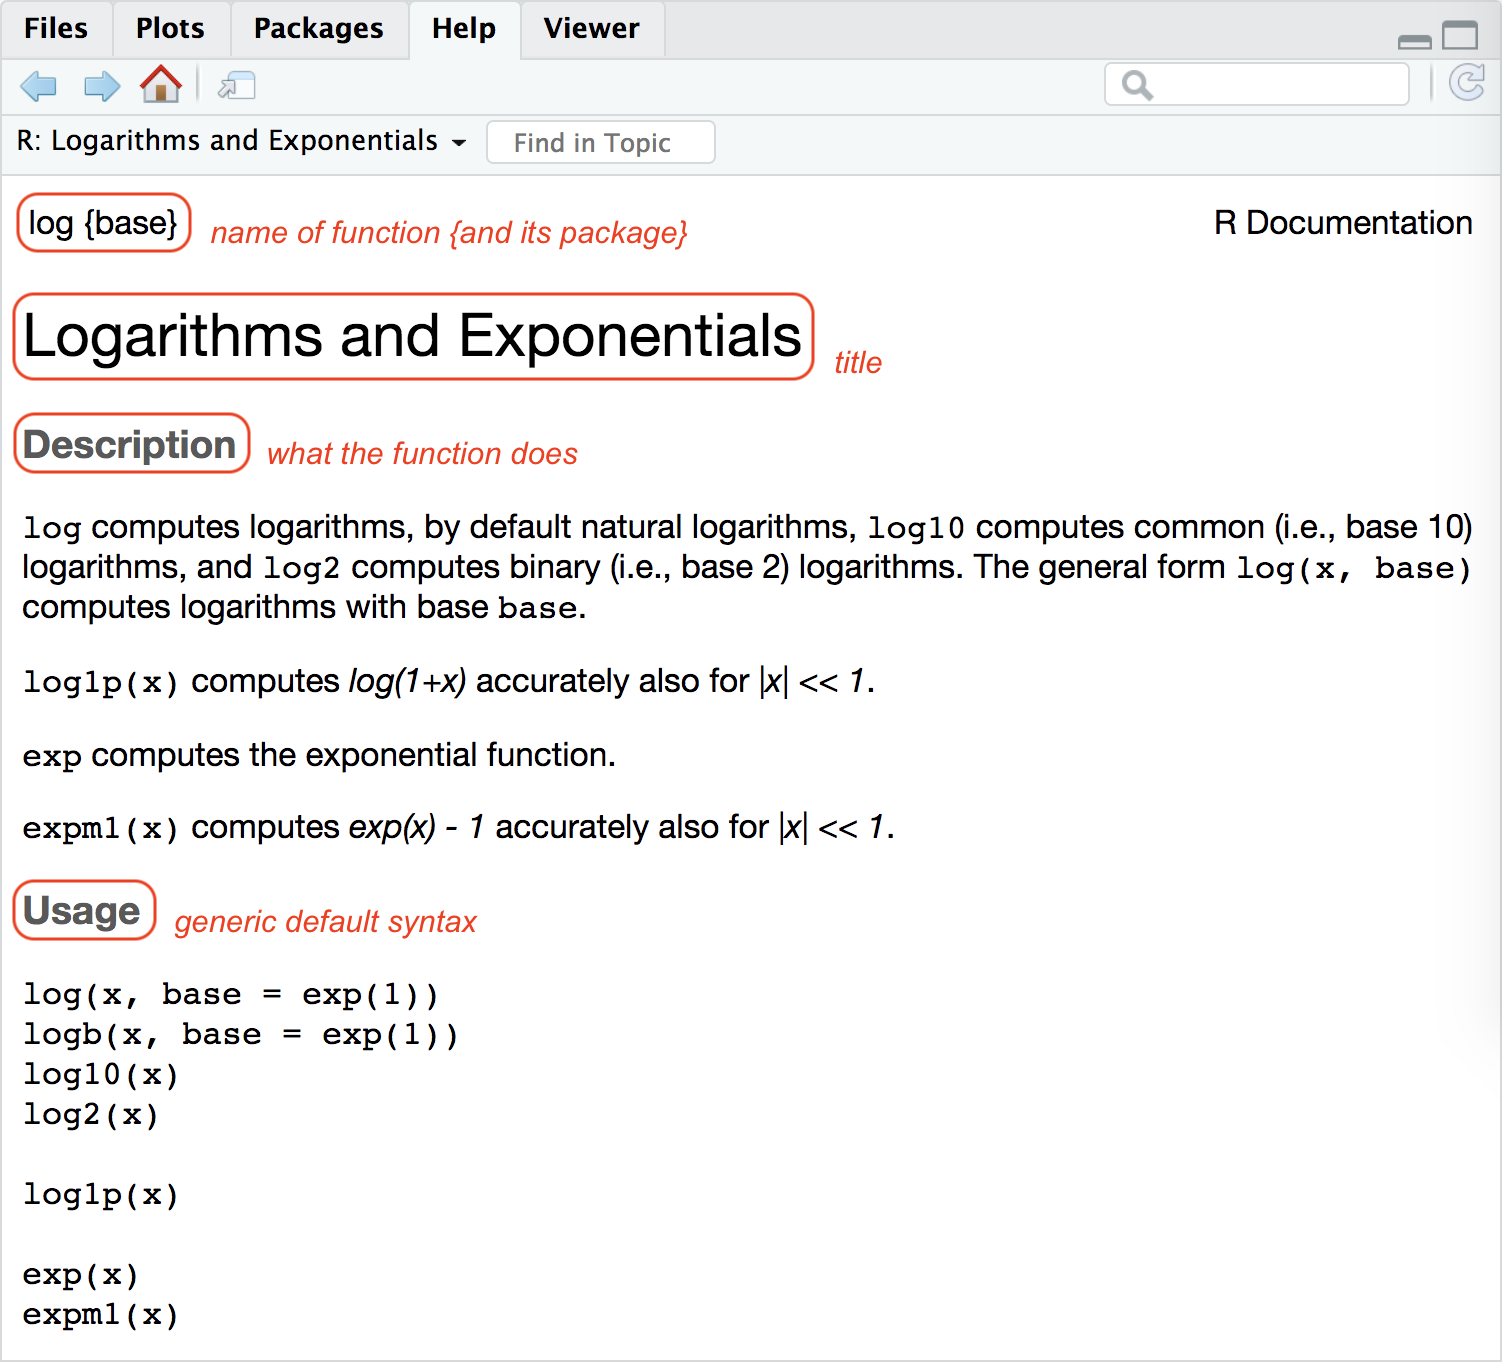
\includegraphics[width=0.85\linewidth]{images/rstudio/help-log-1} 

}

\caption{Help documentation for the log function (part 1)}\label{fig:unnamed-chunk-22}
\end{figure}

\begin{figure}

{\centering 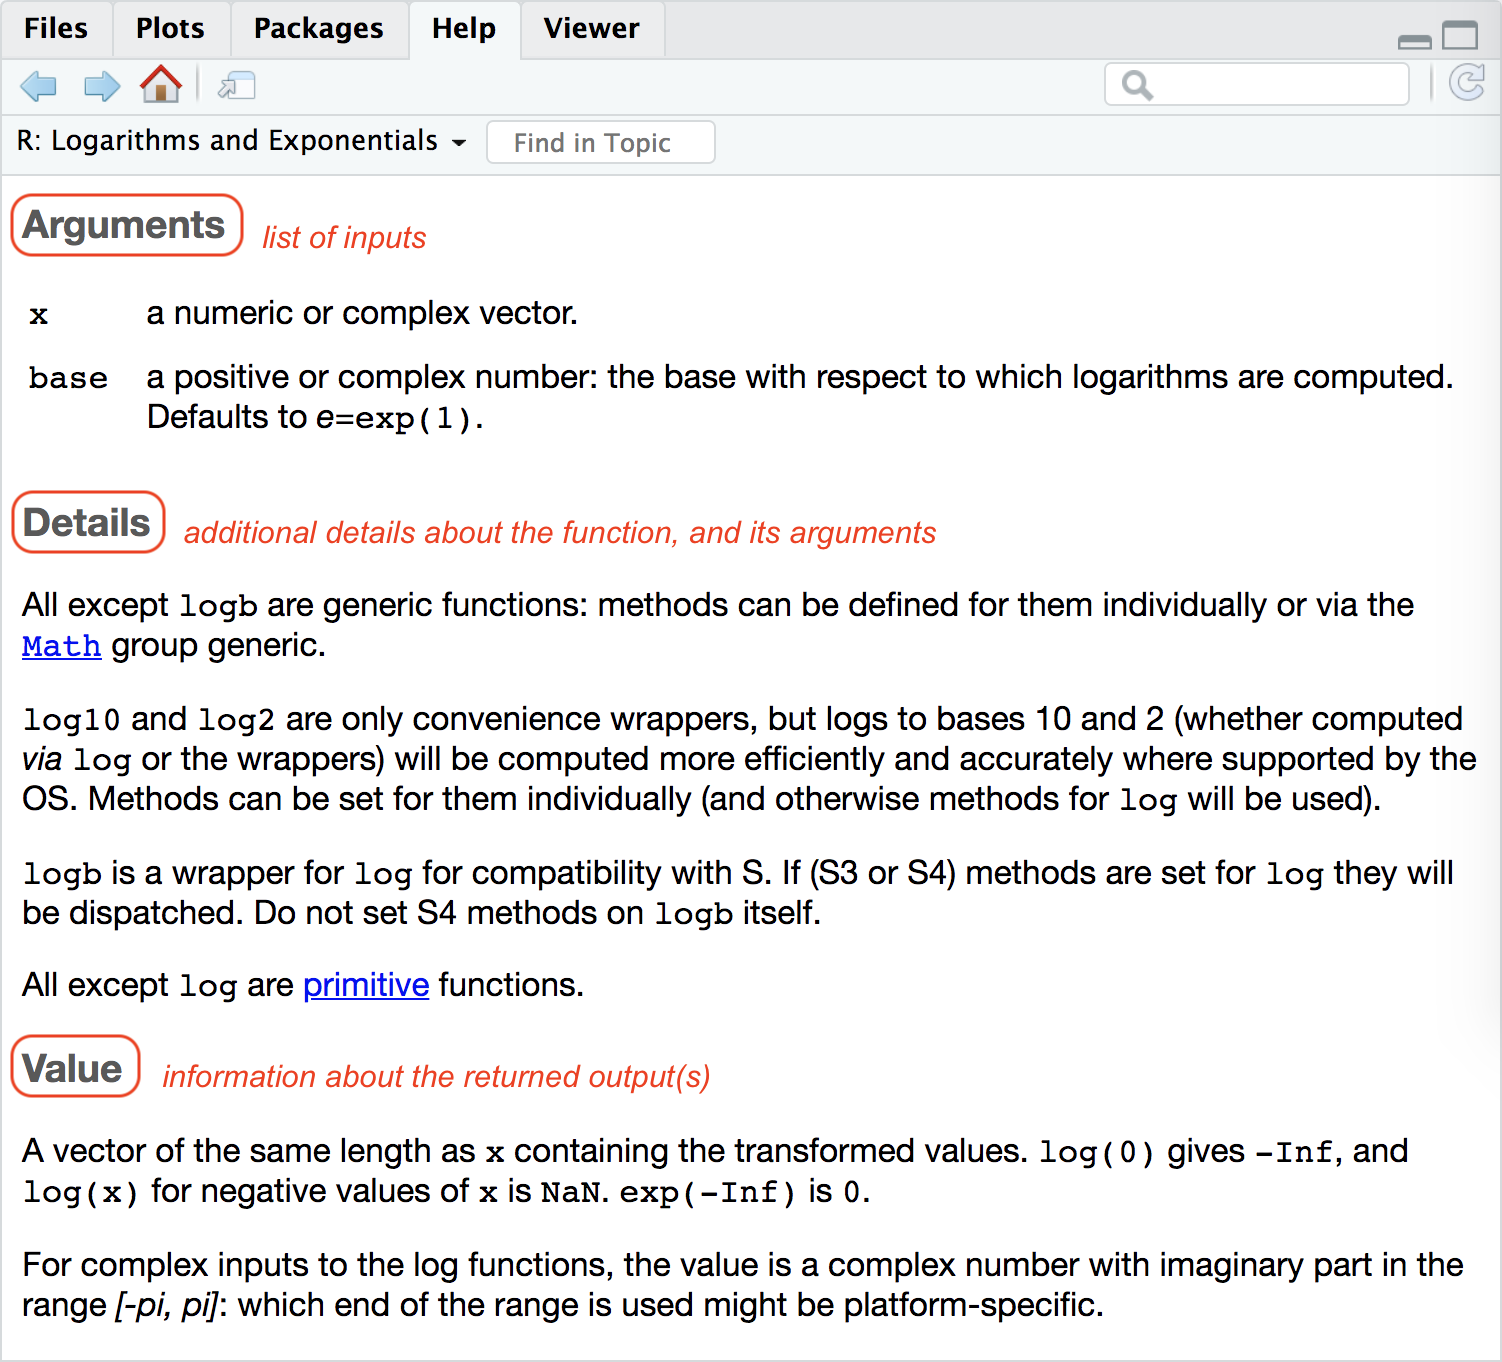
\includegraphics[width=0.85\linewidth]{images/rstudio/help-log-2} 

}

\caption{Help documentation for the log function (part 2)}\label{fig:unnamed-chunk-23}
\end{figure}

\begin{figure}

{\centering 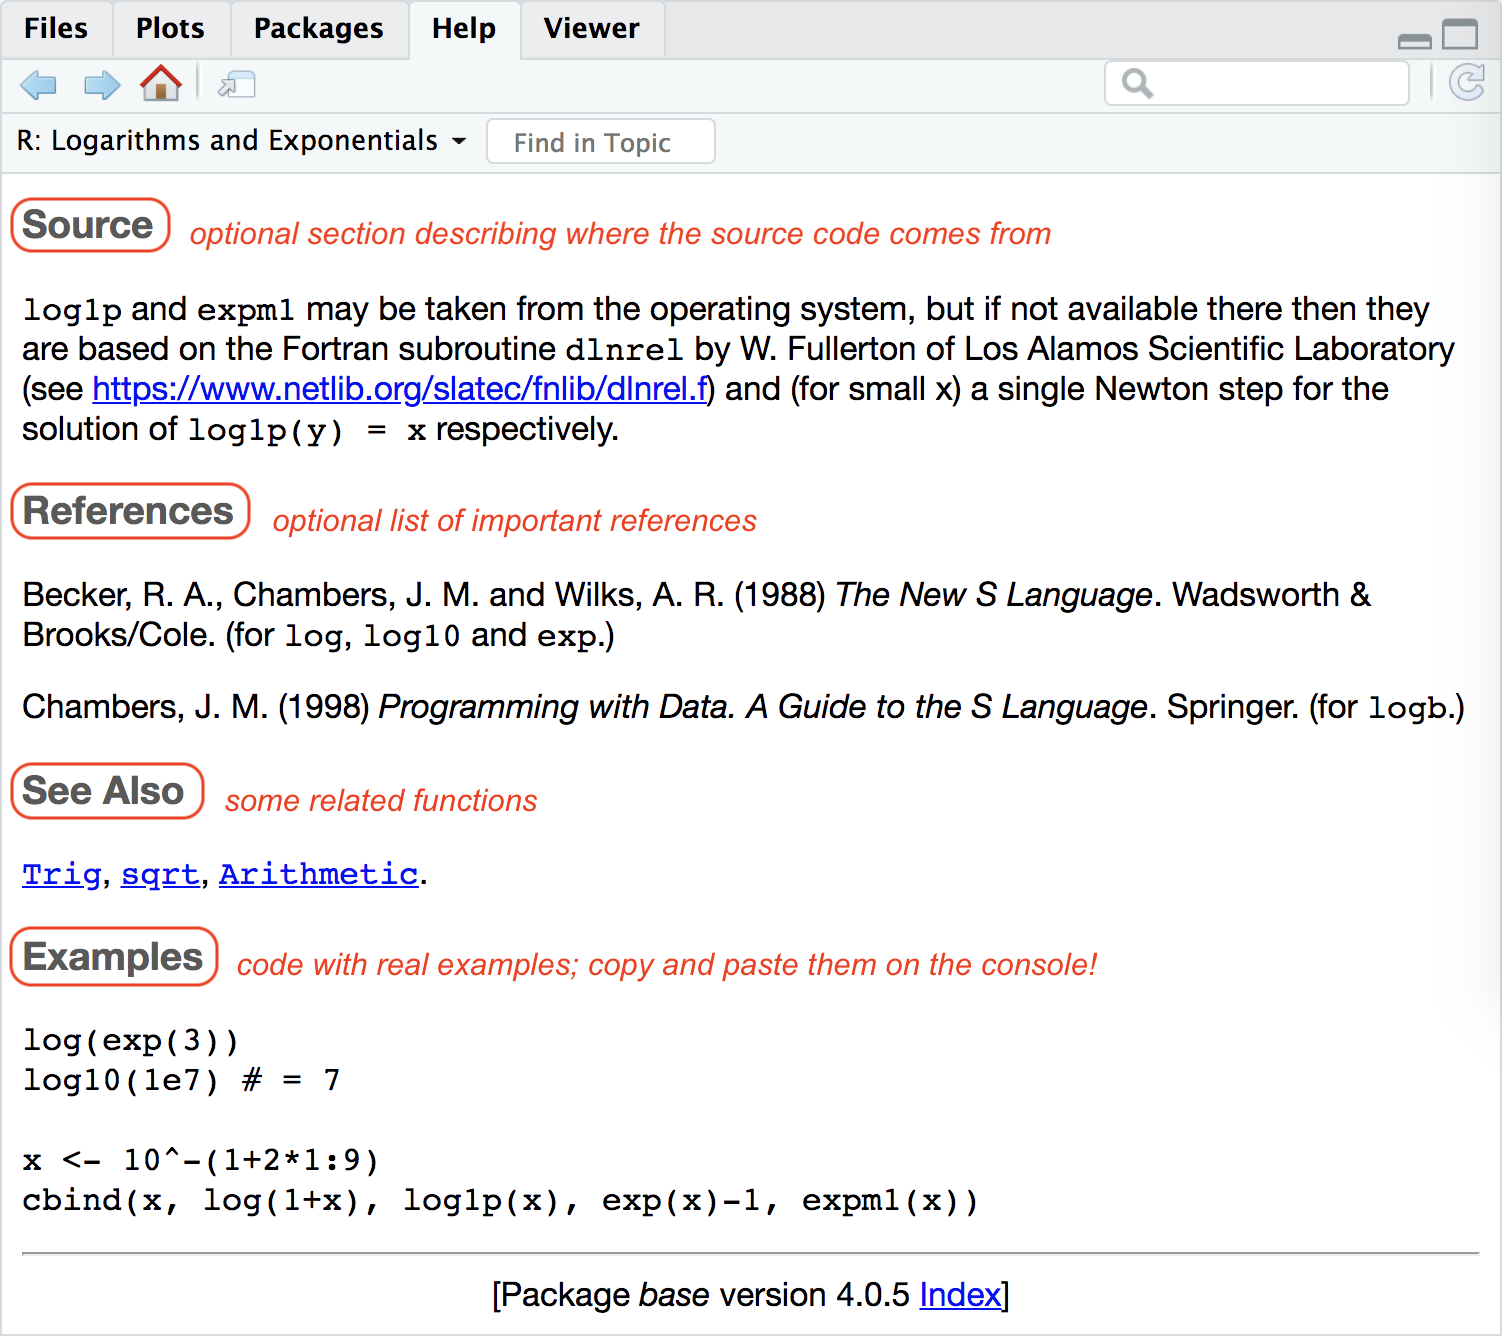
\includegraphics[width=0.85\linewidth]{images/rstudio/help-log-3} 

}

\caption{Help documentation for the log function (part 3)}\label{fig:unnamed-chunk-24}
\end{figure}

\hypertarget{installing-packages}{%
\section{Installing Packages}\label{installing-packages}}

R comes with a large set of functions and packages. A package is a collection
of functions that have been designed for a specific purpose. One of the great
advantages of R is that many analysts, scientists, programmers, and users
can create their own packages and make them available so that everybody can use
them. R packages can be shared in different ways. The most common way to share
a package is to submit it to what is known as \textbf{CRAN}, the
\emph{Comprehensive R Archive Network}.

You can install a package using the \texttt{install.packages()} function. To do this,
I recommend that you \textbf{run this command directly on the console}. In other
words, do not include this command in a source file (e.g.~\texttt{R} script file, \texttt{Rmd}
file). The reason for running this command directly on the console is to avoid
getting an error message when running code from a source file.

To use \texttt{install.packages()} just give it the name of a package, surrounded by
quotes, and R will look for it in CRAN, and if it finds it, R will download it
to your computer.

\begin{Shaded}
\begin{Highlighting}[]
\CommentTok{\# installing (run this on the console!)}
\FunctionTok{install.packages}\NormalTok{(}\StringTok{"knitr"}\NormalTok{)}
\end{Highlighting}
\end{Shaded}

You can also install a bunch of packages at once by placing their names,
each name separated by a comma, inside the \texttt{c()} function:

\begin{Shaded}
\begin{Highlighting}[]
\CommentTok{\# run this command on the console!}
\FunctionTok{install.packages}\NormalTok{(}\FunctionTok{c}\NormalTok{(}\StringTok{"readr"}\NormalTok{, }\StringTok{"ggplot2"}\NormalTok{))}
\end{Highlighting}
\end{Shaded}

Once you installed a package, you can start using its functions by \emph{loading}
the package with the function \texttt{library()}. For better or worse, \texttt{library()}
allows you to specify the name of the package with or without quotes. Unlike
\texttt{install.packages()} you can only specify the name of one package in \texttt{library()}

\begin{Shaded}
\begin{Highlighting}[]
\CommentTok{\# (this command can be included in an Rmd file)}
\FunctionTok{library}\NormalTok{(knitr)      }\CommentTok{\# without quotes}
\FunctionTok{library}\NormalTok{(}\StringTok{"ggplot2"}\NormalTok{)  }\CommentTok{\# with quotes}
\end{Highlighting}
\end{Shaded}

By the way, you only need to install a package once. After a package has been
installed in your computer, the only command that you need to invoke in order
to use its functions is the \texttt{library()} function.

\begin{center}\rule{0.5\linewidth}{0.5pt}\end{center}

\hypertarget{exercises}{%
\section{Exercises}\label{exercises}}

\textbf{1)} Here's the list of monthly expenses for a hypothetical undergraduate
student

\begin{itemize}
\tightlist
\item
  cell phone \$80
\item
  transportation \$20
\item
  groceries \$550
\item
  gym \$15
\item
  rent \$1500
\item
  other \$83
\end{itemize}

\begin{enumerate}
\def\labelenumi{\alph{enumi})}
\item
  Using the \texttt{console} pane of RStudio, create objects (i.e.~variables) for each
  of these expenses listed above, and then create an object \texttt{total} with the sum
  of the expenses.
\item
  Assuming that the student has the same expenses every month, how much would
  she spend during a school ``semester''? (assume the semester involves five months).
  Write code in R to find this value.
\item
  Using the same assumption about the monthly expenses, how much would
  she spend during a school ``year''? (assume the academic year is 10 months).
  Write code in R to find this value.
\end{enumerate}

\textbf{2)} Use the function \texttt{install.packages()} to install packages \texttt{"stringr"},
\texttt{"RColorBrewer"}, and \texttt{"bookdown"}

\textbf{3)} Write code in the console to calculate: \(3x^2 + 4x + 8\) when \(x = 2\)

\textbf{4)} Calculate: \(3x^2 + 4x + 8\) but now with a numeric sequence for \(x\)
using \texttt{x\ \textless{}-\ -3:3}

\textbf{5)} Find out how to look for information about math binary operators
like \texttt{+} or \texttt{\^{}} (without using \texttt{?Arithmetic}). \emph{Tip}: quotes are your friend.

\hypertarget{rstudio}{%
\chapter{A Quick Tour Around RStudio}\label{rstudio}}

As I mentioned in the previous chapter, R comes with a simple built-in graphical
user interface, or \emph{GUI} for short. While you can use this interface to
work with R, it is more convenient if you interact with R using a third party
software such as RStudio.

Technically speaking, RStudio is an IDE which is the acronym for
\emph{Integrated Development Environment}. This is just the fancy name for any
software application that provides comprehensive facilities to programmers for
making their lives easier when writing code and developing programs.

Simply put, you can think of RStudio as a ``workbench'' that gives you an
organized working space for interacting with R, while taking care of many of
the little tasks that can be a hassle.

\hypertarget{first-contact-with-rstudio}{%
\section{First Contact with RStudio}\label{first-contact-with-rstudio}}

When you open RStudio, you should be able to see its layout organized into
quadrants officially called \emph{panes} (or panels).

The very first time you launch RStudio you will only see three panes, like in
the screenshot below.

\begin{figure}

{\centering 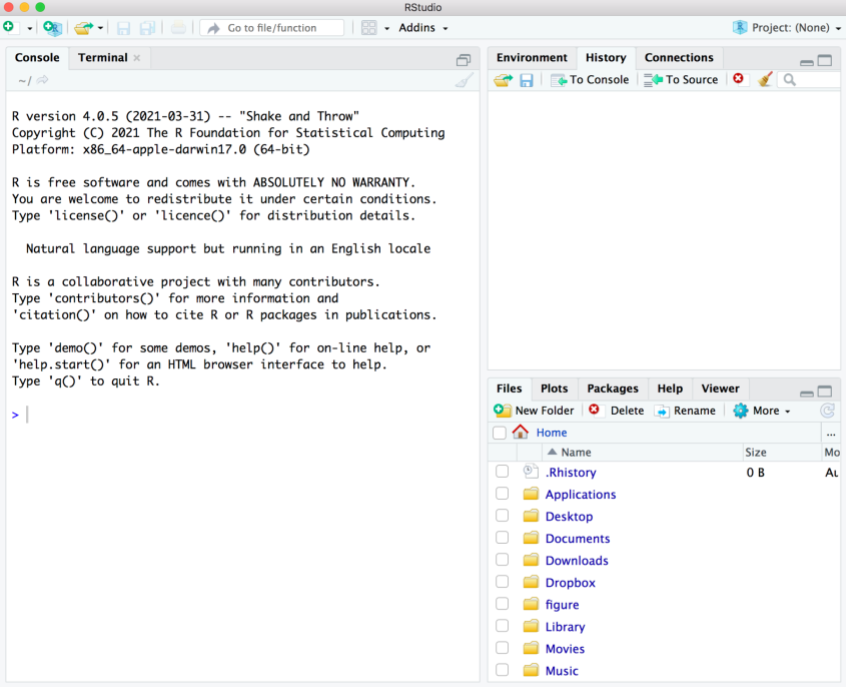
\includegraphics[width=0.7\linewidth]{images/rstudio/rstudio-launch-first-time} 

}

\caption{Screenshot of RStudio when launched for the first time.}\label{fig:unnamed-chunk-26}
\end{figure}

As you can tell from the previous screenshot, the left-hand side shows the
Console pane which is what we used in the previous chapter to write a handful
of simple commands, execute them, and inspect the output provided by R.

If RStudio only displays three panes, why do I call them ``quadrants''? Where is
the fourth pane? Well, to see the extra pane you need to open a file. One
way to do this is by clicking on the icon of a blank file with a green plus sign.
This button is located in the top-left corner of the icons menu bar of RStudio.
A drop-down menu with a long list of available file formats will be displayed,
the first option being an ``R Script'' file (see image below).

\begin{figure}

{\centering 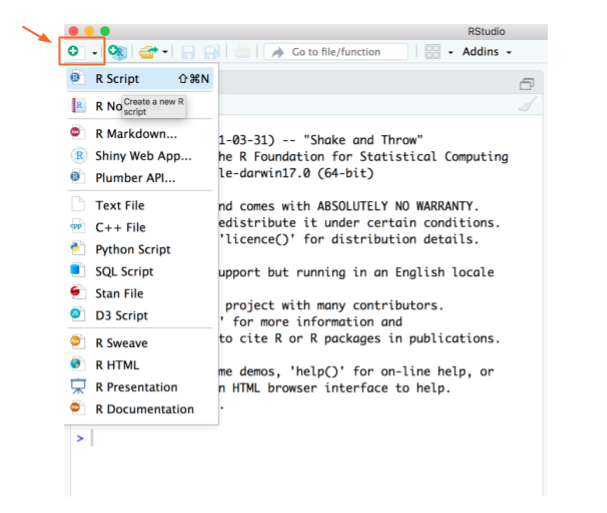
\includegraphics[width=0.7\linewidth]{images/rstudio/rstudio-new-file} 

}

\caption{Opening a new (text) file in RStudio.}\label{fig:unnamed-chunk-27}
\end{figure}

Once you open a (text) file, the layout of RStudio will show the Editor
quadrant, officially called the \emph{Source} pane, like in the following screenshot.

\begin{figure}

{\centering 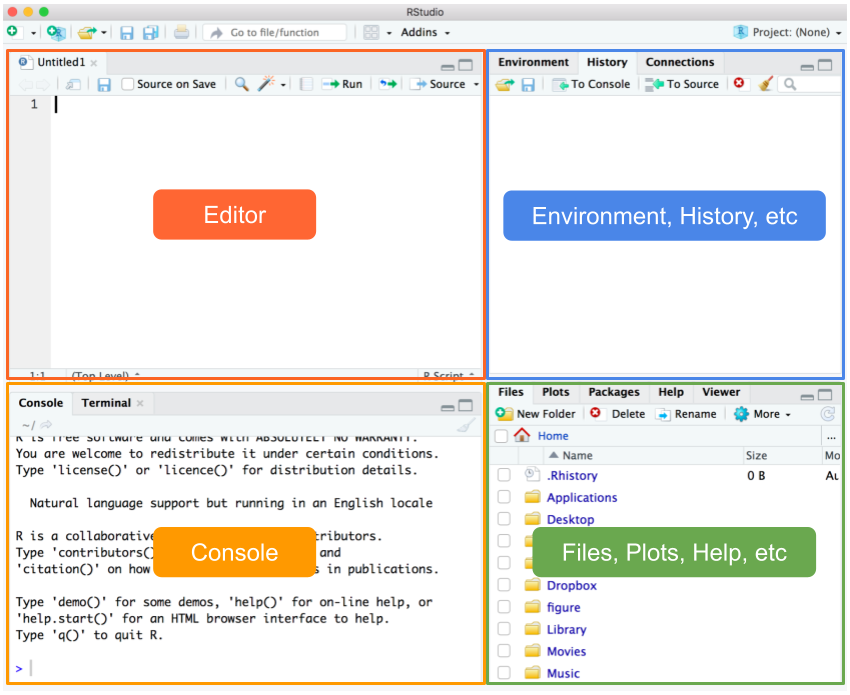
\includegraphics[width=0.8\linewidth]{images/rstudio/rstudio-quadrants} 

}

\caption{RStudio layout organized into quadrants.}\label{fig:unnamed-chunk-28}
\end{figure}

The visual appearance of RStudio's quadrants can be a bit intimidating for
beginners. But fear not. In the above screenshot, the panes are:

\begin{itemize}
\item
  \texttt{Source} or editor pane (top left quadrant)
\item
  \texttt{Console} pane (bottom left quadrant)
\item
  \texttt{Environment/History/Connections} pane (top right quadrant)
\item
  \texttt{Files/Plots/Packages/Help} pane (bottom right quadrant)
\end{itemize}

\textbf{Pro tip:} among many other things, you can change the default location of the panes. If you are interested in knowing what customizing options are available
in RStudio, visit the following link:

\url{https://support.rstudio.com/hc/en-us/articles/200549016-Customizing-RStudio}

If you have no previous programming experience, you don't have to customize
anything right now. It's better if you wait some days until you get a better
feeling of the working environment. You will probably be experimenting (trial
and error) some time with the customizing options until you find what works for
you.

\hypertarget{rstudio-panes-in-a-nutshell}{%
\section{RStudio Panes in a Nutshell}\label{rstudio-panes-in-a-nutshell}}

Sooner or later you will be using all four panes in RStudio. Most programming
activities will require working with both the \texttt{Source} and \texttt{Console} panes.
Certain operations will involve using the \texttt{Files} tab. Occasionally you will
also use one of the tabs in the \texttt{Environment/History/etc} pane. The set of
specific tabs that you have to use really depends on the type of work you plan
to carry out. You will have time to learn the basics---and not so basics---of
every pane throughout the book. The more time you spend in RStudio, and the
more you use it, the more features you will discover about it.

\hypertarget{console}{%
\subsection{Console}\label{console}}

The \texttt{Console} is supposed to be the terminal---or the place---where you type in
commands, which R then executes, and where the output of those commands is
typically displayed. The truth is that most programmers don't write commands
\emph{directly} in the console. Instead, what we use is the \texttt{Source} pane to write
commands in a text file (e.g.~an R-Script file, an R-Markdown file), and then
execute the commands from that pane.

The reason for writing commands in a text file and not directly in the console,
is because of convenience and organization. \emph{Convenience} because, as you will
see, many commands involve writing several lines of code which can be tricky to
write them correctly just by typing in the console. \emph{Organization} in the sense
that having all your commands in a text file makes it easy to store your code,
keep track of all the work you do, build upon it, and share it with others.

So, knowing that programmers rarely make direct use of the \texttt{Console}, when
do you actually use this pane? I don't know about the rest of programmers but
I can tell you how I personally use it.

One common use of the \texttt{Console} is when I want to calculate basic things like
the monthly balance in my credit cards, or the overall score for one of the
students in the classes I teach, or some other quick computation. These are
types of calculations that I could perfectly perform with any scientific
calculator like the one in my smartphone. But more often than not I prefer to
do them in R, typically when that's the tool I have at hand (which happens
almost every day).

The other typical situation in which I use the console is when I'm trying out
some simple idea or testing if a certain command could work. I like to explore
the feasibility of my code with a small example in the console, and then refine
it or generalize it by writing code in a text file---using the \texttt{Source} pane.

\hypertarget{files-plots-packages-help}{%
\subsection{Files, Plots, Packages, Help}\label{files-plots-packages-help}}

The \texttt{Files} quadrant contains multiple tabs.

\begin{itemize}
\item
  \texttt{Files}: this tab lets you navigate your file system without the need of
  leaving RStudio. You can move to any directory or folder in your home directory,
  inspect the contents of a given folder, create a new folder, and perform
  standard operations on files such as opening, renaming, moving, copying, and
  deleting a file. In addition, you can also see the working directory, or change
  to a different directory if you want to.
\item
  \texttt{Plots}: this tab is used by R Graphics Devices to display any graphic or
  image produced by an R plotting function.
\item
  \texttt{Packages}: this tab allows you to install and update R packages. Often, you
  will want to use functions from external R packages, and to do this you must
  first install those packages in your system. While it is possible to write
  commands for doing this, the \texttt{Packages} tab gives you a richer interface to
  see what packages are already available in your computer, what their versions
  are, update them if necessary, or uninstall them in case you no longer need them.
\item
  \texttt{Help}: this is the tab that gives you access to the ``help'' or manual
  documentation of functions, objects, tutorials, and demos of a given R package.
  The \protect\hyperlink{help-documentation}{preceding chapter} contains an example of the
  manual documentation for the \texttt{log()} function, showing the main anatomy of the
  so-called \emph{R Documentation} files.
\end{itemize}

\hypertarget{source-or-editor}{%
\subsection{Source or Editor}\label{source-or-editor}}

The \texttt{Source} pane is basically the text editor of RStudio. This is the quadrant
you use to edit any text file, again, without the need to leave RStudio.
The reason why is called ``source'' is because the text files edited in this
pane are, for the most part, files that contain the commands that R will
run. In other words, these files are the \textbf{source} of the commands to be
executed.

\hypertarget{environment-history-connections}{%
\subsection{Environment, History, Connections}\label{environment-history-connections}}

The last quadrant is the pane that contains, at least, the following three
tabs: \texttt{Environment}, \texttt{History}, and \texttt{Connections}.

I provide a deeper explanation of the \texttt{Environment} and \texttt{History} tabs in the
following chapter \protect\hyperlink{session}{Session Management}. In the meantime, what you
need to know about \texttt{Environment} is that this tab is used to list the objects
that have being created, or that are available, in a given R session.

In turn, the \texttt{History} tab is a very useful resource that lists \textbf{all} the R
commands that you have executed so far. In theory, R will track all the invoked
commands since the first time you used it, unless you've removed the auxiliary
\texttt{.Rhistory} file linked to your working directory, or unless you've modified
the history mechanism used by your R console.

As for the \texttt{Connections} tab, this plays a more advanced (and somewhat obscure)
role that I briefly discuss in part IV of the book.

\begin{center}\rule{0.5\linewidth}{0.5pt}\end{center}

\hypertarget{exercises-1}{%
\section{Exercises}\label{exercises-1}}

\textbf{1)} In RStudio, one of the panes has tabs \texttt{Files,\ Plots,\ Packages,\ Help,\ Viewer}.

\begin{enumerate}
\def\labelenumi{\alph{enumi})}
\tightlist
\item
  In the tab \textbf{Files}, what happens when you click the button with a House icon?
\item
  Go to the \textbf{Help} tab and search for the documentation of the function \texttt{mean}.
\item
  In the tab \textbf{Help}, what happens when you click the button with a House icon?
\end{enumerate}

\textbf{2)} In RStudio, one of the panes has the tabs \texttt{Environment,\ History,\ Connections}.

\begin{enumerate}
\def\labelenumi{\alph{enumi})}
\tightlist
\item
  If you click on tab \textbf{History}, what do see?
\item
  Find what the buttons of the menu bar in tab \textbf{History} are for.
\item
  Likewise, what can you say about the tab \textbf{Environment}?
\end{enumerate}

\textbf{3)} When you start a new R session in Rstudio, a message with similar content to
the text below appears on the console (the exact content will depend on your
R version):

\begin{verbatim}
   R version 3.5.1 (2018-07-02) -- "Feather Spray"
   Copyright (C) 2018 The R Foundation for Statistical Computing
   Platform: x86_64-apple-darwin15.6.0 (64-bit)

   R is free software and comes with ABSOLUTELY NO WARRANTY.
   You are welcome to redistribute it under certain conditions.
   Type 'license()' or 'licence()' for distribution details.

     Natural language support but running in an English locale   

   R is a collaborative project with many contributors.
   Type 'contributors()' for more information and
   'citation()' on how to cite R or R packages in publications.

   Type 'demo()' for some demos, 'help()' for on-line help, or
   'help.start()' for an HTML browser interface to help.
   Type 'q()' to quit R.
\end{verbatim}

\begin{enumerate}
\def\labelenumi{\alph{enumi})}
\item
  What happens when you type (in the console): \texttt{license()}?
\item
  What happens when you type (in the console): \texttt{contributors()}?
\item
  What happens when you type (in the console): \texttt{citation()}?
\item
  What happens when you type (in the console): \texttt{demo()}?
\end{enumerate}

\hypertarget{session}{%
\chapter{Session Management}\label{session}}

In this chapter I review some important aspects about managing your
interactive session with R using RStudio.

Here's what you should always keep in mind. From the point of view of a session,
all the work, activities, and actions you do with R can be classified into
three categories:

\begin{itemize}
\item
  when starting a session
\item
  during the session
\item
  when closing a session
\end{itemize}

Because there are several things going on behind the scenes in each of the
categories listed above, it is important that we talk about them---at least
briefly.

\hypertarget{starting-a-session}{%
\section{Starting a Session}\label{starting-a-session}}

Starting a session can be done in two primary ways:

\begin{itemize}
\item
  launching the R application program, which will give you access to its
  graphical usier interface; or via RStudio or any other IDE that has the
  ability to open an R session.
\item
  by clicking on a file that your computer associates with R (or RStudio).
  For example, R-script files (with file extension \texttt{.R} or \texttt{.r}), R-Markdown
  files (\texttt{.Rmd} extension), R-Noweb files (\texttt{.Rnw} extension), RStudio project
  files (\texttt{.Rproj} extension), etc.
\end{itemize}

\hypertarget{what-happens-when-you-open-an-r-session-via-rstudio}{%
\subsection{What happens when you open an R session via RStudio?}\label{what-happens-when-you-open-an-r-session-via-rstudio}}

This is an important question that many users never stop to think about.
However, it's worth reviewing what happens when a session is started. So let's
talk about this.

\begin{itemize}
\item
  Every time you open RStudio, the console pane will display R's welcome message.
\item
  The console is always linked to a working directory.
\item
  Typically, the working directory of the console will be your home directory,
  unless you specified a different location when you installed R in your computer.
\item
  You can change the working directory to a different directory if you want.
  This change can be permanent (for future sessions), or temporary (for a current
  session).
\item
  To permanently modify the working directory (when a session is opened), go to
  the menu bar, select ``RStudio'' tab, click on ``Preferences'', and modify the
  ``R General'' options.
\item
  To temporarily change the working directory, go to the menu bar, select the
  ``Session'' tab, and click on ``Set Working Directory'', or simply specify a
  working directory with the \texttt{setwd()} function executed from R's console.
\end{itemize}

\hypertarget{opening-a-session-for-the-first-time}{%
\subsection{Opening a session for the first time}\label{opening-a-session-for-the-first-time}}

If you are opening a session in RStudio for the very fist time:

\begin{itemize}
\item
  the ``Editor'' pane will be collapsed, and
\item
  all the tabs in the ``Environment, History, Connections'' pane will be empty
\end{itemize}

In general, when you open a session (\textbf{not} for the very fist time):

\begin{itemize}
\tightlist
\item
  the ``Environment'' tab may display some objects, which means you have some
  existing objects in your global environment. You can also invoke the list
  function \texttt{ls()} to list any available objects in your current session:
\end{itemize}

\begin{Shaded}
\begin{Highlighting}[]
\CommentTok{\# what objects are in my global environment?}
\FunctionTok{ls}\NormalTok{()}
\end{Highlighting}
\end{Shaded}

\begin{itemize}
\tightlist
\item
  the ``History'' tab may contain lines of previously used commands; if this is
  the case it means that there is an associated text file called \texttt{.Rhistory} in
  your working directory. You can also use the \texttt{history()} function to display
  the \emph{Commands History}, that is, all the commands invoked in your interactive
  sessions:
\end{itemize}

\begin{Shaded}
\begin{Highlighting}[]
\CommentTok{\# is my history of commands being tracked?}
\FunctionTok{history}\NormalTok{()}
\end{Highlighting}
\end{Shaded}

\hypertarget{working-directory}{%
\subsection{Working Directory}\label{working-directory}}

If you open R via an application program (e.g.~launching RStudio) that lets
you interact with R's console, your session will have an associated working
directory, sometimes also referred to as the \emph{current} working directory.

When you install R in your computer, during the installation process a default
working directory is assigned to R. By default, this directory is your home
directory. You can check whether this is the case if you run the
\emph{get working directory} function \texttt{getwd()} in your console.

\begin{Shaded}
\begin{Highlighting}[]
\CommentTok{\# run this command in the console to find out }
\CommentTok{\# the working directory of your session}
\FunctionTok{getwd}\NormalTok{()}
\end{Highlighting}
\end{Shaded}

In RStudio, you can also look at the console pane, and inspect the text right
below the \texttt{Console} tab that always displays the working directory of your
session. If you see the symbols \texttt{\textasciitilde{}/} it means that the home directory
(represented by the tilde) is your working directory.

\begin{figure}

{\centering 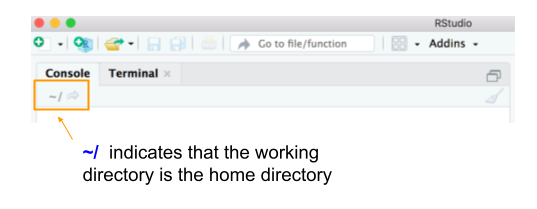
\includegraphics[width=0.7\linewidth]{images/rstudio/rstudio-console-working-directory} 

}

\caption{The working directory is indicated right below the Console tab.}\label{fig:unnamed-chunk-33}
\end{figure}

\hypertarget{working-during-a-session}{%
\section{Working During a Session}\label{working-during-a-session}}

Working with R involves a series of common actions:

\begin{itemize}
\item
  writing commands (in a source document or in the console)
\item
  executing commands (from a source doc or from the console)
\item
  looking or examining outputs
\item
  reading or importing files (e.g.~data files, script files)
\item
  writing or exporting/saving output to files (e.g.~data files, images, results)
\end{itemize}

From the logistical point of vew, it all boils down to executing commands,
taking into account the following:

\begin{itemize}
\item
  where a command is being executed from
\item
  if the command requires an input, where does that input come from?
\item
  if the command produces an output, where does that output go to?
\end{itemize}

This is why we need to describe the following:

\begin{enumerate}
\def\labelenumi{\arabic{enumi}.}
\item
  Working Directory
\item
  Workspace and Global Environment
\item
  History of commands
\end{enumerate}

\hypertarget{sessions-working-directory}{%
\subsection{Session's Working Directory}\label{sessions-working-directory}}

You will be writing commands either directly in the console or in a source
document (e.g.~\texttt{R} script file, \texttt{Rmd} file, etc.)

The console is always associated to a working directory (usually your home
directory).

A source document, once it has been saved, will live in some directory.
\textbf{Ideally}, a source document's directory would be used as its working directory,
using relative file-paths to handle all input and output resources required in
the code of the source document. Unfortunately, this ideal is far from what
happens in practice.

\begin{itemize}
\item
  By default, when you execute code chunks in a \textbf{saved} \texttt{Rmd} file, the
  working directory is the directory where the \texttt{Rmd} file resides in.
\item
  By default, when you execute code from an \texttt{R} file, the working directory
  is that of the console.
\end{itemize}

\hypertarget{workspace-and-global-environment}{%
\subsection{Workspace and Global Environment}\label{workspace-and-global-environment}}

Regardless of where commands are being executed from, R will carry out
all the necessary computations, and objects will be created along the way.

The collection of objects that are being created (\emph{and kept alive}) during a
session are part of what is considered to be your \textbf{workspace}.

At a more technical level, all the objects in your workspace are part of an R
\textbf{environment}. To be more precise, the workspace is the \textbf{Global Environment}.

On the console, if you type \texttt{ls()}, R will display all the available objects
in your workspace.

\begin{Shaded}
\begin{Highlighting}[]
\CommentTok{\# available objects in your workspace}
\FunctionTok{ls}\NormalTok{()}
\end{Highlighting}
\end{Shaded}

You can also go to the pane ``Environment, History, \ldots{}'' and
click on the \texttt{Environment} tab to see the objects in your workspace which are
displayed by default under the option ``Global Environment''.

\hypertarget{commands-history}{%
\subsection{Commands History}\label{commands-history}}

When you start a session, R will track all the commands that you execute during
that session. As you execute commands, they will become part of what is called
the \textbf{Commands History}.

You can find the list of all used commands in the \texttt{History} tab,
located in the \emph{Environment, History, Connections} pane of RStudio. You can
also access the commands history with the function \texttt{history()}.

\begin{figure}

{\centering 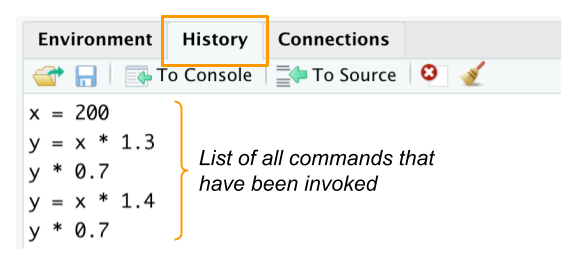
\includegraphics[width=0.65\linewidth]{images/rstudio/rstudio-history-tab} 

}

\caption{The comands history is avaialble in the History tab.}\label{fig:unnamed-chunk-35}
\end{figure}

By default, the history of commands are stored in a text file called \texttt{.Rhistory}
that is saved in your session's working directory.

\hypertarget{closing-a-session}{%
\section{Closing a Session}\label{closing-a-session}}

At some point, the work that you've done in a session will come to an end, and
consequently you will \textbf{close} the session.

When closing a session, what should you do?

This is a somewhat ``very personal'' type of question, because it is up to you to
decide what should happen to all the work that you've done in R.

Having said that, you can always decide whether or not to:

\begin{itemize}
\item
  save changes in your source document(s)
\item
  save the commands history in a text file
\item
  save the objects in your workspace (i.e.~objects in Global Environment) in
  a binary file (native to R)
\end{itemize}

It turns out that RStudio comes with default actions that take place
when you close a session:

\begin{itemize}
\item
  it will ask you if you want to save changes in your source documents
\item
  it will ask you if you want to save the workspace in an \texttt{.RData} file
  (this is a file that uses R's native binary format; this is saved in your
  session's working directory)
\item
  it will automatically save your commands history in a text file called
  \texttt{.Rhistory} (saved in your session's working directory)
\end{itemize}

Also, because of RStudio's default settings, the next time you open a new
session it will:

\begin{itemize}
\item
  restore the previously open source document
\item
  restore objects in the \texttt{.RData} file into your workspace
\item
  give you access to all the commands stored in the \texttt{.Rhistory} file
\end{itemize}

Of course, you can change and customize the default settings of RStudio so
that R/RStudio do certain things when closing a session.

\hypertarget{rmdfiles}{%
\chapter{Intro to R Markdown Files}\label{rmdfiles}}

Most of the times you won't be working directly on the console.
Instead, you will be typing your commands in some \textbf{source file}.
The most basic type of source files are known as \emph{R script files}.
But there are more flavors of source files. A very convenient type of source
file that allow you to mix R code with narrative is an \textbf{R markdown file}
commonly referred to as \texttt{Rmd} file.

\hypertarget{get-to-know-rmd-files}{%
\section{\texorpdfstring{Get to know \texttt{Rmd} files}{Get to know Rmd files}}\label{get-to-know-rmd-files}}

In the menu bar of RStudio, click on \textbf{File}, then \textbf{New File},
and choose \textbf{R Markdown}. Select the default option (Document),
and click \textbf{Ok}.

\textbf{Rmd} files are a special type of file, referred to as a \emph{dynamic document},
that allows to combine narrative (text) with R code. Because you will
be turning in most homework assignments as \texttt{Rmd} files, it is important
that you quickly become familiar with this resource.

Locate the button \textbf{Knit HTML} (the one with a knitting icon) and click on it
so you can see how \texttt{Rmd} files are rendered and displayed as HTML documents.

\hypertarget{what-is-an-rmd-file}{%
\subsection{\texorpdfstring{What is an \texttt{Rmd} file?}{What is an Rmd file?}}\label{what-is-an-rmd-file}}

\textbf{Rmd} files are a special type of file, referred to as a \emph{dynamic document}.
This is the fancy term we use to describe a document that allows us to combine
narrative (text) with R code in one single file.

\emph{R markdown} files use a special syntax called \textbf{markdown}. To be more precise,
Rmd files let you type text using either: 1) R syntax for code that needs to be
executed; 2) markdown syntax to write your \emph{narrative}, and 3) latex syntax for
math equations and symbols.

Rmd files are plain text files. This means that you can open an Rmd file
with any text editor (not just RStudio) and being able to see and edit its
contents.

The main idea behind dynamic documents is simple yet very powerful: instead of
working with two separate files, one that contains the R code, and
another one that contains the narrative, you use an \texttt{.Rmd} file to include
both the commands and the narrative.

One of the main advantages of this paradigm,
is that you avoid having to copy results from your computations and paste them
into a report file. In fact, there are more complex ways to work with dynamic
documents and source files. But the core idea is the same: combine narrative
and code in a way that you let the computer do the manual, repetitive,
and time consuming job.

Rmd files is just one type of dynamic document that you will find in RStudio.
In fact, RStudio provides other file formats that can be used
as dynamic documents: e.g.~\texttt{.Rnw}, \texttt{.Rpres}, \texttt{.Rhtml}, etc.

\hypertarget{anatomy-of-an-rmd-file}{%
\subsection{\texorpdfstring{Anatomy of an \texttt{Rmd} file}{Anatomy of an Rmd file}}\label{anatomy-of-an-rmd-file}}

The structure of an \texttt{.Rmd} file can be divided in two parts: 1) a \textbf{YAML header},
and 2) the \textbf{body} of the document. In addition to this structure, you should
know that \texttt{.Rmd} files use three types of syntaxes: YAML, Markdown, and R.

The \emph{YAML header} consists of the first few lines at the top of the file.
This header is established by a set of three dashes \texttt{-\/-\/-} as delimiters
(one starting set, and one ending set). This part of the file requires you
to use YAML syntax (Yet Another Markup Language.)
Within the delimiter sets of dashes, you specify settings (or metadata) that
will apply to the entire document. Some of the common
options are things like:

\begin{itemize}
\tightlist
\item
  \texttt{title}
\item
  \texttt{author}
\item
  \texttt{date}
\item
  \texttt{output}
\end{itemize}

The \emph{body} of the document is everything below the YAML header. It consists
of a mix of narrative and R code. All the text that is narrative is written
in a markup syntax called \textbf{Markdown} (although you can also use LaTeX math
notation). In turn, all the text that is code
is written in R syntax inside \emph{blocks of code}.

There are two types of blocks of code: 1) \textbf{code chunks}, and
2) \textbf{inline code}. Code chunks are lines of text separated from any lines of
narrative text. Inline code is code inserted within a line of narrative text .

\hypertarget{how-does-an-rmd-file-work}{%
\subsection{How does an Rmd file work?}\label{how-does-an-rmd-file-work}}

Rmd files are plain text files. All that matters is the syntax of its content.
The content is basically divided in the header, and the body.

\begin{itemize}
\tightlist
\item
  The header uses YAML syntax.
\item
  The narrative in the body uses Markdown syntax.
\item
  The code and commands use R syntax.
\end{itemize}

The process to generate a nice rendered document from an Rmd file is
known as \textbf{knitting}. When you \emph{knit} an Rmd file, various R packages
and programs run behind the scenes. But the process can be broken down
in three main phases: 1) Parsing, 2) Execution, and 3) Rendering.

\begin{enumerate}
\def\labelenumi{\arabic{enumi})}
\tightlist
\item
  Parsing: the content of the file is parsed (examined line by line)
  and each component is identified as yaml header, or as markdown text, or as R code.
\end{enumerate}

Each component receives a special treatment and formatting.

The most interesting part is in the pieces of text that are R code.
Those are separated and executed if necessary. The commands may be included
in the final document. Also, the output may be included in the final document.
Sometimes, nothing is executed nor included.

Depending on the specified output format (e.g.~HTML, pdf, word), all the
components are assembled, and one single document is generated.

\hypertarget{yet-another-syntax-to-learn}{%
\subsection{Yet Another Syntax to Learn}\label{yet-another-syntax-to-learn}}

R markdown (\texttt{Rmd}) files use \href{https://daringfireball.net/projects/markdown/}{markdown}
as the main syntax to write content. Markdown is a very lightweight type of
markup language, and it is relatively easy to learn.

One of the most common sources of confusion when learning about R and Rmd
files has to do with the hash symbol \texttt{\#}. As you know, \texttt{\#} is the character
used by R to indicate comments. The issue is that the \texttt{\#} character has a
different meaning in markdown syntax. Hashes in markdown are used to define
levels of headings.

In an Rmd file, a hash \texttt{\#} that is inside a code chunk will be treated as
an R comment. A hash outside a code chunk, will be treated as markdown syntax,
making its associated text a given type of heading.

\hypertarget{code-chunks}{%
\section{Code chunks}\label{code-chunks}}

There are dozens of options available to control the executation of the code,
the formatting and display of both the commands and the output, the display
of images, graphs, and tables, and other fancy things. Here's a list of the
basic options you should become familiar with:

\begin{itemize}
\tightlist
\item
  \texttt{eval}: whether the code should be evaluated

  \begin{itemize}
  \tightlist
  \item
    \texttt{TRUE}
  \item
    \texttt{FALSE}
  \end{itemize}
\item
  \texttt{echo}: whether the code should be displayed

  \begin{itemize}
  \tightlist
  \item
    \texttt{TRUE}
  \item
    \texttt{FALSE}
  \item
    numbers indicating lines in a chunk
  \end{itemize}
\item
  \texttt{error}: whether to stop execution if there is an error

  \begin{itemize}
  \tightlist
  \item
    \texttt{TRUE}
  \item
    \texttt{FALSE}
  \end{itemize}
\item
  \texttt{results}: how to display the output

  \begin{itemize}
  \tightlist
  \item
    \texttt{markup}
  \item
    \texttt{asis}
  \item
    \texttt{hold}
  \item
    \texttt{hide}
  \end{itemize}
\item
  \texttt{comment}: character used to indicate output lines

  \begin{itemize}
  \tightlist
  \item
    the default is a double hash \texttt{\#\#}
  \item
    \texttt{""} empty character (to have a cleaner display)
  \end{itemize}
\end{itemize}

\hypertarget{resources-for-markdown}{%
\subsection{Resources for Markdown}\label{resources-for-markdown}}

In RStudio's menu bar select the \texttt{Help} tab. Then click on the option
\texttt{Markdown\ Quick\ Reference}.

Work through the markdown tutorial:
www.markdown-tutorial.com

Your turn: After lab discussion, find some time to go through this
additional markdown tutorial
www.markdowntutorial.com

RStudio has a very comprehensive R Markdown tutorial:
Rstudio markdown tutorial

  \bibliography{book.bib}

\end{document}
